\documentclass[11pt, twoside, pdftex]{article}


\newcommand{\typeName}{Verilog}
\newcommand{\edition}{Standard}
%%%%%%%%%%%%%%%%%%%%%%%%%
% Preamble
% This include all the settings that we should use for the document

\newcommand{\PDFTitle}{Quartus\textsuperscript{\textregistered} Prime Introduction Using \typeName{} Designs}
\newcommand{\commonPath}{../../../Common}
\newcommand{\datePublished}{Mar 2022}

\newcommand{\versnum}{21.1} %version number quartus/AMP
\newcommand{\quartusname}{Quartus\textsuperscript{\textregistered} Prime}	
\newcommand{\textBar}{For \quartusname{} \versnum{}}
\newcommand{\thisyear}{2022 } %for copyright
\newcommand{\company}{FPGAcademy.org}
\newcommand{\longteamname}{FPGAcademy.org}
\newcommand{\teamname}{FPGAcademy}
\newcommand{\website}{FPGAcademy.org}

\newcommand{\productAcronym}{AMP}
\newcommand{\productNameShort}{Monitor Program}

\newcommand{\productNameMedTM}{Monitor Program}
\newcommand{\productNameMed}{Monitor Program}

%\newcommand{\headerLogoFilePath}[1]{#1/FPGAcademy.png}



\setlength\topmargin{-0.25in}
\setlength\headheight{0in}
\setlength\headsep{0.35in}
\setlength\textheight{8.5in}
\setlength\textwidth{7in}
\setlength\oddsidemargin{-0.25in}
\setlength\evensidemargin{-0.25in}
\setlength\parindent{0.25in}
\setlength\parskip{0in} 

\pdfpagewidth 8.5in
\pdfpageheight 11in

% listings is a package that supports encapsulating source code in LaTeX conveniently

\usepackage{listings}
% add support for graphics
\usepackage{graphicx}
\usepackage[usenames, dvipsnames]{color}

\def\expandparam\lstinputlisting[#1]#2{\edef\tmp{\noexpand\lstinputlisting[#1]{#2}}\tmp}

\widowpenalty 10000
\clubpenalty 10000

%%%%%%%%%%%%%%%%%%%% Source Code Formatting %%%%%%%%%%%%%%%%%%%%
\definecolor{globalCommentColour}{rgb}{0.588,0.588,0.588}

%%%%%%%%%%%%%%%%%%%%%%%%%%%%%%%%%%%%%%%%%%%%%%%%%%%%
% Defining a NiosII ASM highlighter for lstlisting
\lstdefinelanguage[NiosII]{Assembler} {
 	morekeywords={add, addi, and, andhi, andi, beq, bge, bgeu, bgt, bgtu, ble,  bleu, blt, bltu, bne, br, break,% 
 	bret, call, callr, cmpeq, cmpeqi, cmpge, cmpgei, cmpgeu, cmpgeui, cmpgt, cmpgti, cmpgtu, cmpgtui, cmple,%
 	cmplei, cmpleu, cmpleui, cmplt, cmplti, cmpltu, cmpltui, cmpne, cmpnei, custom, div, divu, eret, flushd,%
 	flushda, flushi, flushp, initd, initda, initi, jmp, jmpi, ldb, ldbio, ldbu, ldbuio, ldh, ldhio, ldhu, ldhuio,%
 	ldw, ldwio, mov, movhi, movi, movia, movui, mul, muli, mulxss, mulxsu, mulxuu, nextpc, nop, nor, or, orhi, ori,%
 	rdctl, rdprs, ret, rol, roli, ror, sll, slli, sra, srai, srl, srli, stb, stbio, sth, sthio, stw, stwio,%
 	sub, subi, sync, trap, wrctl, wrtcl, wrprs, xor, xori, xorhi, xori},% 	
 	morekeywords=[2]{.abort, .ABORT, .align, .app-file, .ascii, .asciz, .balign, .byte, .comm, .data, .def,%
 	.desc, .dim, .double, .eject, .else, .end, .endef, .endif, .equ, .equiv, .err, .extern, .file, .fill, .float,%
 	.global, .globl, .hword, .ident, .if, .include, .int, .irp, .irpc, .lcomm, .lflags, .line, .linkonce, .ln,%
 	.list, .long, .macro, .mri, .nolist, .octa, .org, .p2align, .psize, .quad, .rept, .sbttl, .scl, .section,%
 	.set, .short, .single, .size, .sleb128, .skip, .space, .stadb, .stabn, .stabs, .string, .symver, .tag,%
 	.text, .title, .type, .val, .uleb128, .word},% 	
 	morekeywords=[3]{et, bt, gp, sp, fp, ea, sstatus, ra, pc, status, estatus, bstatus, ienable, ipending, cpuid,%
 	exception, pteaddr, tlbacc, tlbmisc, eccinj, badaddr, config, mpubase, mpuacc},% 	
 	sensitive=t,%
 	alsoletter=.,%
	morestring=[b]",%
 	morecomment=[s]{/*}{*/},%
 	morecomment=[l]\#,%
   }[keywords,comments,strings]
   
   %% NOTE: morekeywords=[2] are GNU directives.
   
   \definecolor{niosInstructionColour}{rgb}{0.000,0.608,0.000}
   \definecolor{niosDirectiveColour}{rgb}{0.000,0.000,0.902}
   \definecolor{niosSpecialRegColour}{rgb}{0.000,0.000,0.000}
   \definecolor{niosStringColour}{rgb}{0.808,0.482,0.000}
   
   %% NOTE: To make bold use: =\bfseries\color{<colour>}
   \lstdefinestyle{defaultNiosStyle} {
   language=[NiosII]{Assembler},
   stringstyle=\color{niosStringColour},
   keywordstyle=\color{niosInstructionColour},
   keywordstyle=[2]\color{niosDirectiveColour},
   keywordstyle=[3]\itshape\color{niosSpecialRegColour}
   }
%%%%%%%%%%%%%%%%%%%%%%%%%%%%%%%%%%%%%%%%%%%%%%%%%%%%

%%%%%%%%%%%%%%%%%%%%%%%%%%%%%%%%%%%%%%%%%%%%%%%%%%%%
% Defining a ArmA9 ASM highlighter for lstlisting
\lstdefinelanguage[ArmA9]{Assembler} {
 	morekeywords={ADC, ADD, ADDS, AND, ANDS, B, BAL, BEQ, BGE, BGT, BL, BLT, BIC, BKPT, BLX, BNE, BX, CDP, CLZ, CMN, CMP, EOR,%
 	EORS, LDC, LDM, LDR, LDRB, LDRBT, LDRH, LDRSB, LDRSH, LDRT, LSL, MCR, MLA, MOV, MOVW, MOVT, MRC, MRS, MSR, MUL, MVN, ORR, PLD,%
 	ROR, RSB, RSC, SBC, SMLAL, SMULL, STC, STM, STR, STRB, STRBT, STRH, STRT, SUB, SUBS, SWI, SWP, SWPB, TEQ, UMLAL,
 	PUSH, POP, MOVS, RORS, LSR},%
 	morekeywords=[2]{.abort, .ABORT, .align, .app-file, .ascii, .asciz, .balign, .byte, .comm, .data, .def,%
 	.desc, .dim, .double, .eject, .else, .end, .endef, .endif, .equ, .equiv, .err, .extern, .file, .fill, .float,%
 	.global, .globl, .hword, .ident, .if, .include, .int, .irp, .irpc, .lcomm, .lflags, .line, .linkonce, .ln,%
 	.list, .long, .macro, .mri, .nolist, .octa, .org, .p2align, .psize, .quad, .rept, .sbttl, .scl, .section,%
 	.set, .short, .single, .size, .sleb128, .skip, .space, .stadb, .stabn, .stabs, .string, .symver, .tag,%
 	.text, .title, .type, .val, .vectors, .uleb128, .word},%
 	morekeywords=[3]{SP, PC, MIDR, CTR, TCMTR, TLBTR, MPIDR, ID_PFR0, ID_PFR1, ID_DFR0, ID_MMFR0, ID_MMFR1, ID_MMFR2,%
 	ID_MMFR3, ID_ISAR0, ID_ISAR1, ID_ISAR2, ID_ISAR3, ID_ISAR4, CCSIDR, CLIDR, AIDR, CSSELR, TTBR0, TTRB1, TTBR2, DACR,%
 	DFSR, IFSR, ADFSR, AIFSR, DFAAR, IFAR, ICIALLUIS, BPIALLIS, PAR, ICIALLU, ICIMVAU, BPIALL, DCIMVAC, DCISW, V2PCWPR,%
 	DCCVAC, DCCSW, DDIMVAC, DCISW, TLBALLIS, TLBIMVAIS, TLBIASIDIS, TLBIMVAAIS, TLBIALL, TLBIMVA, TLBIASID, TLBIMVAA,%
 	PMCR, PMCNTENSET, PMCNTENCLR, PMOVSR, PMSWINC, PMSELR, PMXEVTYPER, PMXEVCNTR, PMUSERENR, PMINTENSET, PMINTENCLR,%
 	PRRR, NRRR, PLEIDR, PLEASR, PLEFSR, PLEUAR, PLEPCR, VBAR, MVBAR, ISR, FCSEIDR, CONTEXTIDR, TPIDRURW, TPIDRURO, TPIDRPRW},%
 	sensitive=f,%
 	alsoletter=.,%
	morestring=[b]",%
 	morecomment=[s]{/*}{*/},%
 	morecomment=[l]{//},%
   }[keywords,comments,strings]
   
   %% NOTE: morekeywords=[2] are GNU directives.
   
   \definecolor{armInstructionColour}{rgb}{0.000,0.608,0.000}
   \definecolor{armDirectiveColour}{rgb}{0.000,0.000,0.902}
   \definecolor{armSpecialRegColour}{rgb}{0.000,0.000,0.000}
   \definecolor{armStringColour}{rgb}{0.808,0.482,0.000}
   
   \lstdefinestyle{defaultArmStyle} {
   language=[ArmA9]{Assembler},
   stringstyle=\color{armStringColour},
   keywordstyle=\color{armInstructionColour},
   keywordstyle=[2]\color{armDirectiveColour},
   keywordstyle=[3]\itshape\color{armSpecialRegColour}
   }
%%%%%%%%%%%%%%%%%%%%%%%%%%%%%%%%%%%%%%%%%%%%%%%%%%%%

%%%%%%%%%%%%%%%%%%%%%%%%%%%%%%%%%%%%%%%%%%%%%%%%%%%%
% Defining style for the verilog.

\definecolor{verilogCommentColour}{rgb}{0.000,0.502,0.000}

\lstdefinestyle{defaultVerilogStyle} {
language={Verilog},
keywordstyle=\color{blue},
commentstyle=\color{verilogCommentColour}
}
%%%%%%%%%%%%%%%%%%%%%%%%%%%%%%%%%%%%%%%%%%%%%%%%%%%%

%%%%%%%%%%%%%%%%%%%%%%%%%%%%%%%%%%%%%%%%%%%%%%%%%%%%
% Defining style for the vhdl.
\lstdefinestyle{defaultVHDLStyle} {
language={VHDL},
keywordstyle=\color{blue},
commentstyle=\color{verilogCommentColour}
}
%%%%%%%%%%%%%%%%%%%%%%%%%%%%%%%%%%%%%%%%%%%%%%%%%%%%

%%%%%%%%%%%%%%%%%%%%%%%%%%%%%%%%%%%%%%%%%%%%%%%%%%%%
% Java
\definecolor{javaStringColour}{rgb}{0.808,0.482,0}
%%%%%%%%%%%%%%%%%%%%%%%%%%%%%%%%%%%%%%%%%%%%%%%%%%%%

%%%%%%%%%%%%%%%%%%%%%%%%%%%%%%%%%%%%%%%%%%%%%%%%%%%%
% Defining language styles
% C
\definecolor{CStringColour}{rgb}{0.808,0.482,0}
%%%%%%%%%%%%%%%%%%%%%%%%%%%%%%%%%%%%%%%%%%%%%%%%%%%%

%%%%%%%%%%%%%%%%%%%%%%%%%%%%%%%%%%%%%%%%%%%%%%%%%%%%
% Defining extended LaTeX language.
\lstdefinelanguage[LocalLaTeX]{TeX}[LaTeX]{TeX}%
 	{moretexcs={bf, it, sf, lstset},%
   	}%

\lstdefinestyle{defaultLocalLatexStyle} {
language=[LocalLatex]{TeX},
keywordstyle=\color{blue}\bfseries,
keywordstyle=[2]\color{blue},
keywordstyle=[3]\color{blue}\bfseries
}
%%%%%%%%%%%%%%%%%%%%%%%%%%%%%%%%%%%%%%%%%%%%%%%%%%%%

\lstset{
%language = C,
%language = Verilog,
%basicstyle=\color{black}\rmfamily\ttfamily,
basicstyle=\small\color{black}\ttfamily,
commentstyle=\small\color{globalCommentColour}\itshape\ttfamily,
keywordstyle=\small\color{blue}\bfseries\ttfamily,
showstringspaces=false,
frame=none, %lines % boxed listings
breaklines=true,
breakatwhitespace=true,
tabsize=4
}
%%%%%%%%%%%%%%%%%%%%%%%%%%%%%%%%%%%%%%%%%%%%%%%%%%%%%%%%%%%%%%%%


%\usepackage[centering]{geometry}.
%%%%%%%%%%%%%%%%%%%%%%%%%%%%%%%%%%%%%%%%%%%%%%%%%%%
% Document Settings
\usepackage[labelsep=period]{caption}
% we can choose a better font later
%\usepackage{palatino}
\usepackage{fourier}
%\fontencoding{T1}
% include common used symbols
\usepackage{textcomp}
% add support for graphics
\usepackage{graphicx}
\usepackage[usenames, dvipsnames]{color}
% enable to draw thick or thin table hlines
\setlength{\doublerulesep}{\arrayrulewidth}
\usepackage{longtable}
\setlongtables
%\usepackage{array}
% It may be better to use PDFLaTeX as it can generate bookmarks for the
% document

% Add some useful packages
\usepackage{ae,aecompl}
\usepackage{epsfig,float,times}

% reset the font for section
\usepackage{sectsty}
%\allsectionsfont{\fontfamily{ptm}\selectfont}
\allsectionsfont{\usefont{OT1}{phv}{bc}{n}\selectfont}

% use compact space for sections
\usepackage[compact]{titlesec}
\titlespacing{\section}{0pt}{0.2in}{*0}
\titlespacing{\subsection}{0pt}{0.1in}{*0}
\titlespacing{\subsubsection}{0pt}{0.05in}{*0}

% fancyhdr header and footer customization
\usepackage{layout}
\usepackage{fancyhdr}
\pagestyle{fancy}
\fancyhead{}
\fancyhead[R]{\textit{\tiny{\textBar}}}
\fancyfoot{}
\fancyfoot[LO,
RE]{\textrm{\href{https://www.fpgacademy.org}{\small \longteamname}} \\ {\small \datePublished }}
\fancyfoot[RO, LE]{\small \thepage}
% two-side settings
%\fancyhead{} % clear all header fields
%\fancyfoot{} % clear all footer fields
%\fancyfoot[LE,RO]{\thepage}
\renewcommand{\headrulewidth}{2pt}
\renewcommand{\headrule}{{\color{blue} \hrule width\headwidth height\headrulewidth \vskip-\headrulewidth}}
\renewcommand{\footrulewidth}{0pt}

% Format the footer on page 1
\fancypagestyle{plain}{
\fancyhead{}
\fancyfoot{}
\fancyfoot[LO,
RE]{\textrm{\href{https://www.fpgacademy.org}{\small \longteamname}} \\ {\small \datePublished }}
\fancyfoot[RO, LE]{\small \thepage}
\renewcommand{\headrulewidth}{0pt}
}
% adjust some setting to try to make the figure stay in the same page with text
% Reference: 	http://www.cs.uu.nl/~piet/floats/node1.html
%   			http://mintaka.sdsu.edu/GF/bibliog/latex/floats.html
%   General parameters, for ALL pages:
\renewcommand{\topfraction}{0.9}	% max fraction of floats at top
\renewcommand{\bottomfraction}{0.8}	% max fraction of floats at bottom
%   Parameters for TEXT pages (not float pages):
\setcounter{topnumber}{3}
\setcounter{bottomnumber}{3}
\setcounter{totalnumber}{5}     % 2 may work better
\setcounter{dbltopnumber}{2}    % for 2-column pages
\renewcommand{\dbltopfraction}{0.9}	% fit big float above 2-col. text
\renewcommand{\textfraction}{0.07}	% allow minimal text w. figs
%   Parameters for FLOAT pages (not text pages):
\renewcommand{\floatpagefraction}{0.7}	% require fuller float pages
% N.B.: floatpagefraction MUST be less than topfraction !!
\renewcommand{\dblfloatpagefraction}{0.7}	% require fuller float pages
%%%%%%%%%%%%%%%%%%%%%%%%%%%%%%%%%%%%%%%%%%%%%%%%%%%
% remember to use [htp] or [htpb] for placement
%%%%%%%%%%%%%%%%%%%%%%%%%%%%%%%%%%%%%%%%%%%%%%%%%%%

% set no indent for paragraph
\setlength{\parindent}{0em}
\addtolength{\parskip}{11pt}
\newcommand{\compact}{[topsep=0pt]}
% use this package to reduce space
\usepackage{enumitem}
\usepackage{multirow}
\usepackage{rotating}
\usepackage{pifont}
\usepackage{dingbat}
\newcommand{\itemsecond}{$\circ$}
%
%%%%%%%%%%%%%%%%%%
\date{}
\author{}
%%%%%%%%%%%%%%%%%%
\newcommand{\de}{DE-series}
\newcommand{\up}{FPGAcademy}
\newcommand{\fabric}{Avalon Switch Fabric}
\newcommand{\TODO}[1]{\textcolor{red}{\textbf{TODO}: #1}}
\def\registered{{\ooalign{\hfil\raise .00ex\hbox{\scriptsize R}\hfil\crcr\mathhexbox20D}}}

% enable url and reference(bookmarks) in pdf
\usepackage{url}
\usepackage[pdftex, colorlinks]{hyperref}
\hypersetup{%
pdftitle={\PDFTitle},
linkcolor=blue,
hyperindex=true,
pdfauthor={\longteamname},
pdfkeywords={FPGAcademy, Academic Program, Example System},
bookmarksnumbered,
bookmarksopen=false,
filecolor=blue,
pdfstartview={FitH},
urlcolor=blue,
plainpages=false,
pdfpagelabels=true,
linkbordercolor={1 1 1} %no color for link border
}%
%%%%%%%%%%%%%%%%%%%%%%%%%%%%%%%%%%%%%%%%%%%%%%%%%%%
\setlength{\fboxsep}{0.7pt}
\setlength{\fboxrule}{0.5pt}

\newcommand{\red}[1]{{\color{red}\sf{#1}}}
\newcommand{\blue}[1]{{\color{blue}\sf{#1}}}




%%%%%%%%%%%%%%%%%%%%%%%%%
% Add title
\newcommand{\doctitle}{Quartus\textsuperscript{\textregistered} Prime Introduction \\ Using \typeName{} Designs}
\newcommand{\dochead}{Quartus\textsuperscript{\textregistered} Prime Introduction Using \typeName{} Designs}
% Usually no need to change these two lines
\title{\fontfamily{phv}\selectfont{\doctitle} }
\chead{ \small{\textsc{\bfseries \dochead} } }
% Customizations
%%%%%%%%%%%%%%%%%%%%%%%%%
% Allows multiple figures per page

\renewcommand\floatpagefraction{.9}
\renewcommand\topfraction{.9}
\renewcommand\bottomfraction{.9}
\renewcommand\textfraction{.1}   
\setcounter{totalnumber}{50}
\setcounter{topnumber}{50}
\setcounter{bottomnumber}{50}
\raggedbottom

%%%%%%%%%%%%%%%%%%%%%%%%%

%%%%%%%%%%%%%%%%%%%%%%%%%
% Document Begings
\begin{document}

%%%%%%%%%%%%%%%%%%%%%%%%%
% Header Logo and Title
\begin{table}

    \centering
    \begin{tabular}{p{5cm}p{4cm}}
        \hspace{-3cm}
        &
        \raisebox{1\height}{\parbox[h]{0.5\textwidth}{\Large\fontfamily{phv}\selectfont{\textsf{\doctitle}}}}
    \end{tabular}
    \label{tab:logo}
\end{table}

\colorbox[rgb]{0,0.384,0.816}{\parbox[h]{\textwidth}{\color{white}\textsf{\textit{\textBar}}}}

\thispagestyle{plain}
%%%%%%%%%%%%%%%%%%%%%%%%%

%%%%%%%%%%%%%%%%%%%%%%%%%
% Table of Contents
{\tiny \tableofcontents}
\newpage
%%%%%%%%%%%%%%%%%%%%%%%%%

%%%%%%%%%%%%%%%%%%%%%%%%%
% Introduction
\section{Introduction}


This tutorial presents an introduction to the Quartus\textsuperscript{\textregistered} Prime CAD system.
It gives a general overview of a typical CAD flow for designing circuits that are
implemented by using FPGA devices, and shows how this flow is realized in
the Quartus Prime software. The design process is illustrated by giving step-by-step
instructions for using the Quartus Prime software to implement a very simple circuit
in an Intel\textsuperscript{\textregistered} FPGA device.

The Quartus Prime system includes full support for all of the popular methods of
entering a description of the desired circuit into a CAD system. This tutorial
makes use of the \typeName{} design entry method, in which the user specifies the desired
circuit in the \typeName{} hardware description language. 
Three versions of this tutorial are available; one
uses the Verilog hardware description language, another uses the VHDL hardware description language, and the third is based on defining
the desired circuit in the form of a schematic diagram.

The last step in the design process involves configuring the designed circuit
in an actual FPGA device. To show how this is done, it is assumed that the user has access
to the Intel DE-series Development and Education board connected to 
a computer that has Quartus Prime software installed. 
A reader who does not have access to the DE-series board will still find the tutorial useful
to learn how the FPGA programming and configuration task is performed.

The screen captures in the tutorial were obtained using the 
Quartus Prime version \versnum \ \edition{} Edition; other versions of the software may be slightly different.

%%%%%%%%%%%%%%%%%%%%%%%%%

%%%%%%%%%%%%%%%%%%%%%%%%%
% Background
\newpage


\section{Background}
Computer Aided Design (CAD) software makes it easy to implement a desired logic
circuit by using a programmable logic device, such as a Field-Programmable 
Gate Array (FPGA) chip. A typical FPGA CAD flow is illustrated in Figure~\ref{fig:1}. 

\begin{figure}[H]
   \begin{center}
      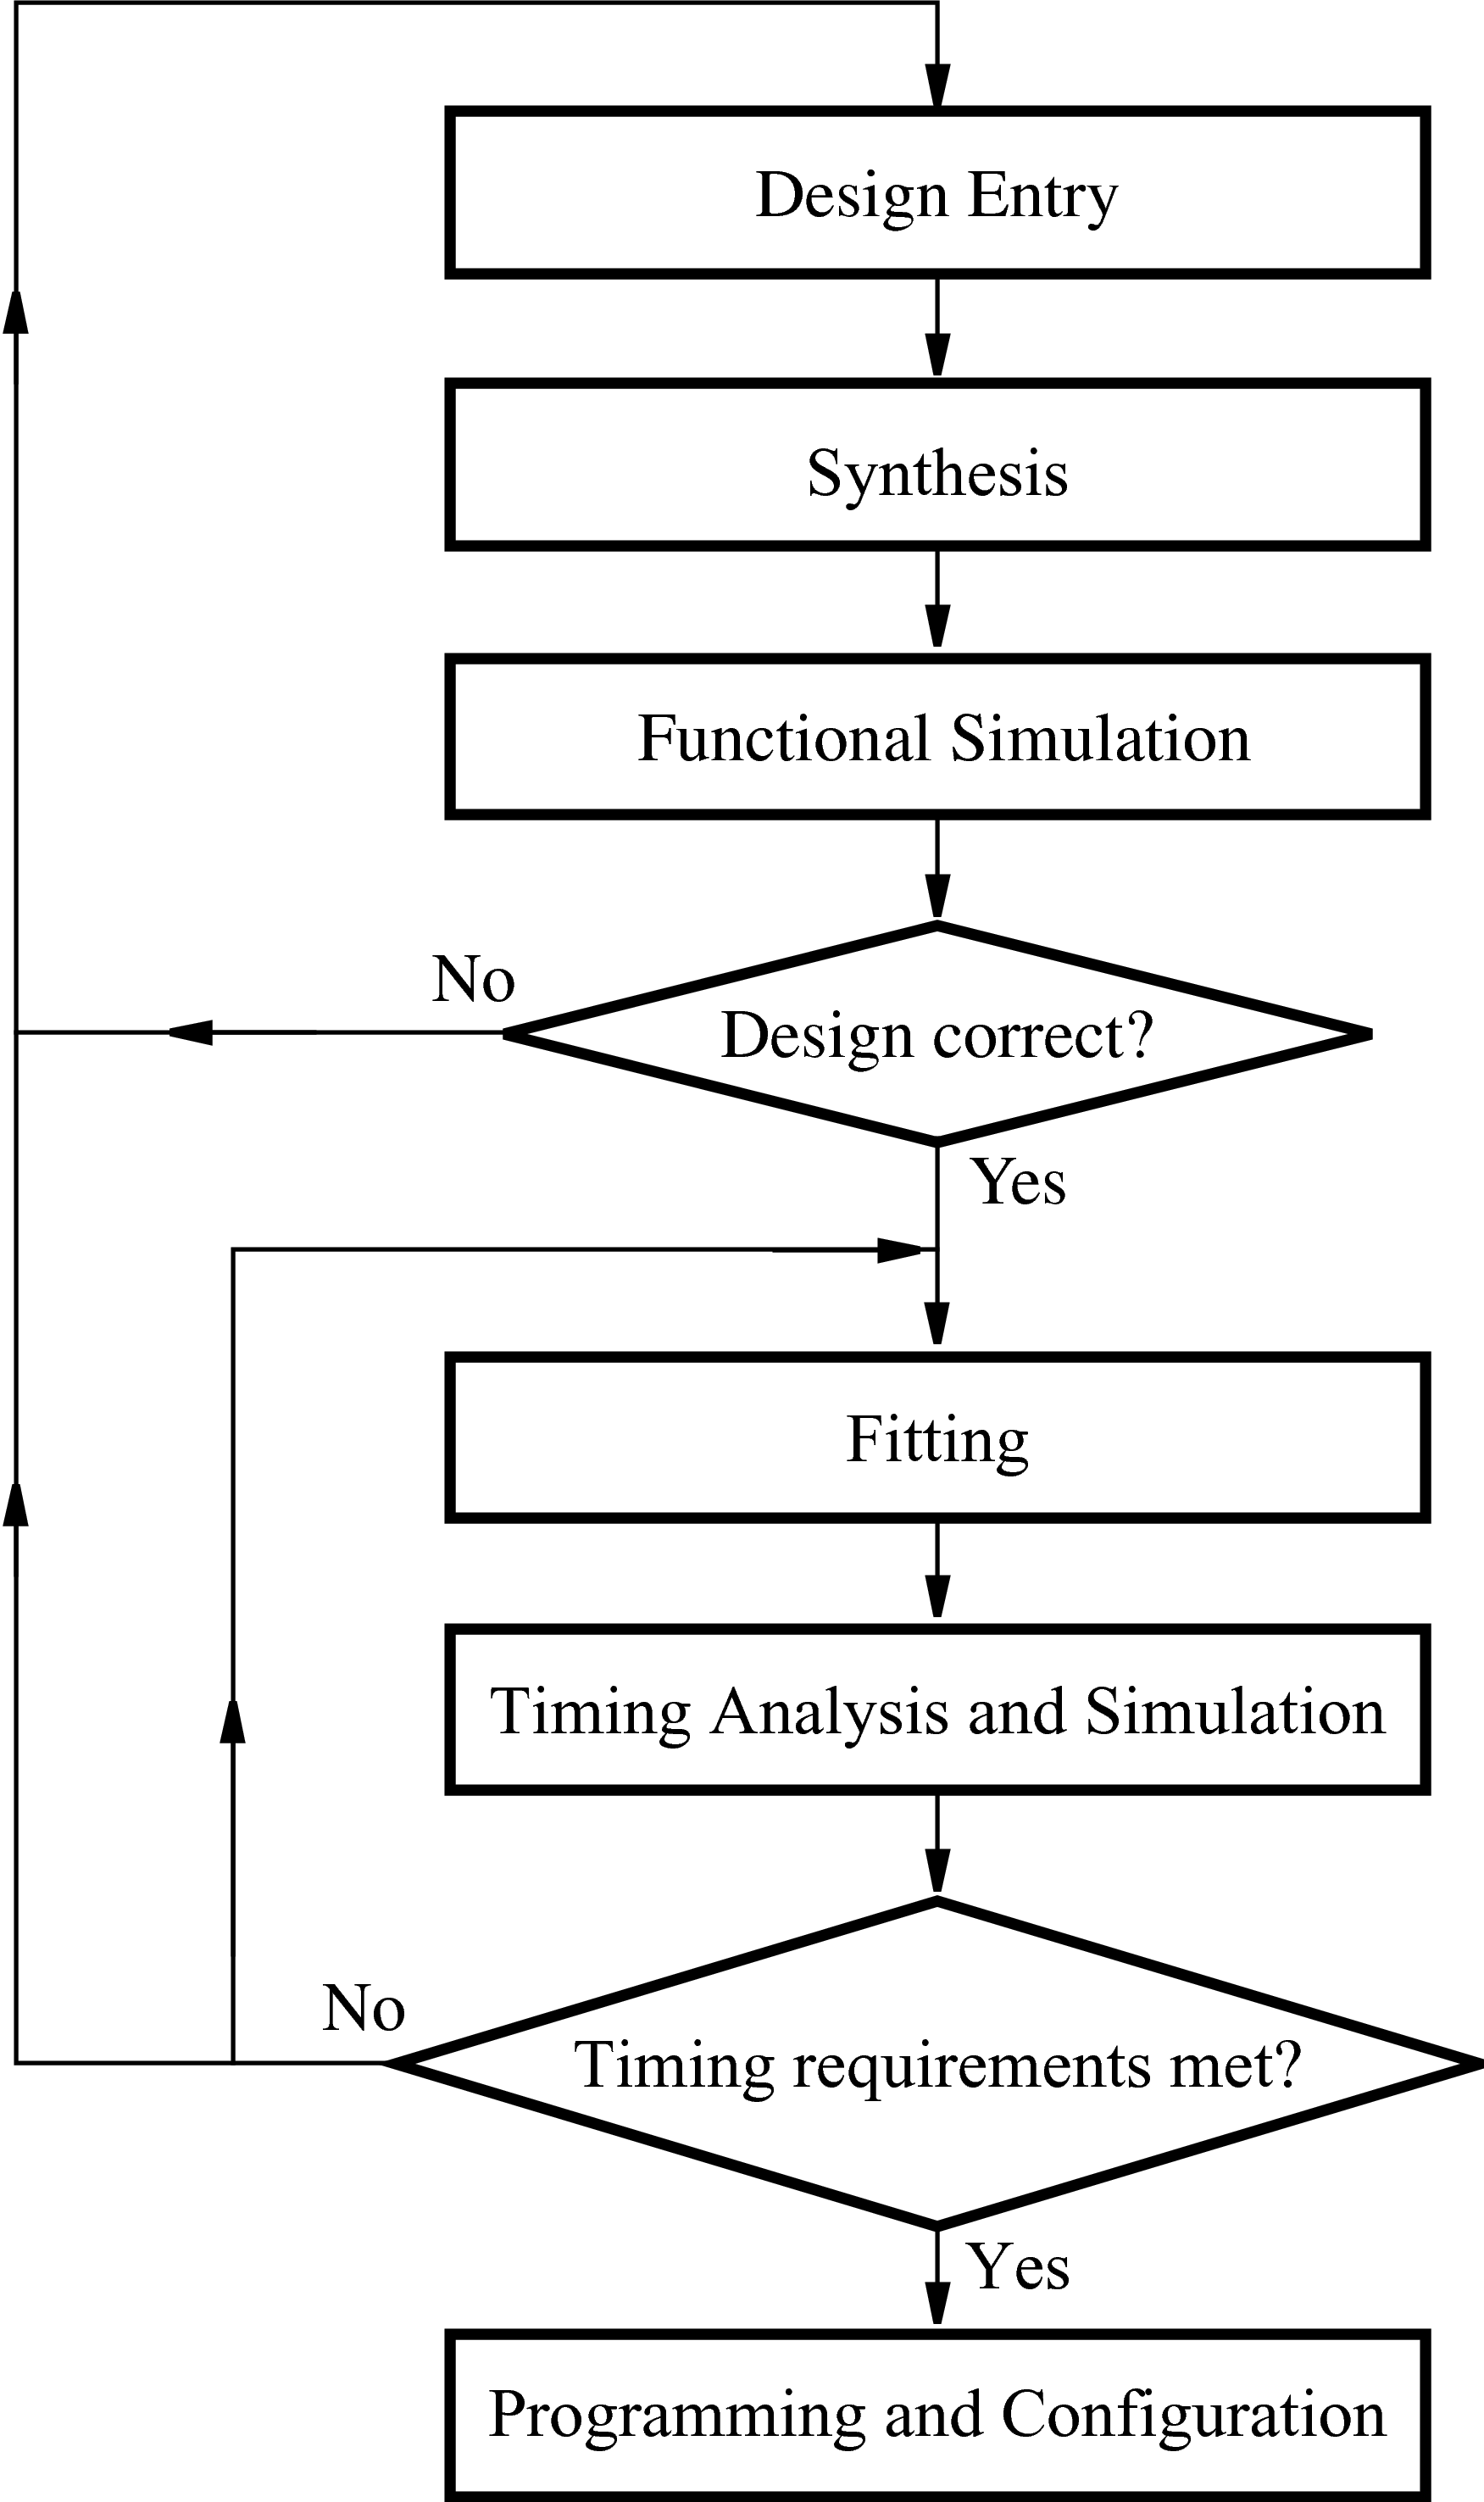
\includegraphics[scale=1]{figures/figure1.png}
   \caption{Typical CAD flow.} 
	 \label{fig:1}
	 \end{center}
\end{figure}

The CAD flow involves the following steps:
\begin{itemize}
\item {\bf Design Entry} -- the desired circuit is specified either by means of
a schematic diagram, or by using a hardware description language, 
such as Verilog or VHDL
\item {\bf Synthesis} -- the entered design is synthesized into a circuit
that consists of the logic elements (LEs) provided in the FPGA chip
\item {\bf Functional Simulation} -- the synthesized circuit is tested to
verify its functional correctness; this simulation does not take into account
any timing issues
\item {\bf Fitting} -- the CAD Fitter tool determines the placement of the LEs 
defined in the netlist into the LEs in an actual FPGA chip; it also 
chooses routing wires in the chip to make the required connections 
between specific LEs 
\item {\bf Timing Analysis} -- propagation delays along the various paths
in the fitted circuit are analyzed to provide an indication of the expected
performance of the circuit
\item {\bf Timing Simulation} -- the fitted circuit is tested to verify both
its functional correctness and timing
\item {\bf Programming and Configuration} -- the designed circuit is implemented
in a physical FPGA chip by programming the configuration switches that configure
the LEs and establish the required wiring connections
\end{itemize}

\noindent
This tutorial introduces the basic features of the Quartus Prime software. 
It shows how the software can be used to design and implement a circuit specified by
using the \typeName{} hardware description language.
It makes use of the graphical user interface to invoke the Quartus Prime commands.
Doing this tutorial, the reader will learn about:
\begin{itemize}
\item Creating a project
\item Design entry using \typeName{} code
\item Synthesizing a circuit specified in \typeName{} code
\item Fitting a synthesized circuit into an Intel FPGA
\item Assigning the circuit inputs and outputs to specific pins on the FPGA
\item Simulating the designed circuit
\item Programming and configuring the FPGA chip on Intel's DE-series board
\end{itemize}

%%%%%%%%%%%%%%%%%%%%%%%%%

%%%%%%%%%%%%%%%%%%%%%%%%%
% Getting Started
\section{Getting Started}

\noindent 
Each logic circuit, or subcircuit, being designed with Quartus Prime software is
called a {\it project}. The software works on one project at a time
and keeps all information for that project in a single directory (folder) in
the file system.
To begin a new logic circuit design, the first step is
to create a directory to hold its files. 
To hold the design files for this tutorial, we will use a directory 
{\it introtutorial}.
The running example for this tutorial is a simple circuit for two-way light control.

Start the Quartus Prime software. You should see a display
similar to the one in Figure~\ref{fig:2}. This display consists of several windows that 
provide access to all the features of 
Quartus Prime software, which the user selects with the computer mouse.
Most of the commands provided by Quartus Prime software can be accessed by using a set of
menus that are located below the title bar. For
example, in Figure~\ref{fig:2} clicking the left mouse button on the menu
named {\sf File} opens the menu shown in Figure~\ref{fig:3}. Clicking the
left mouse button on the entry {\sf Exit} exits
from Quartus Prime software. In general, whenever the mouse is used to select
something, the {\it left} button is used. Hence we will not normally
specify which button to press. In the few cases when it is
necessary to use the {\it right} mouse button, it will be specified explicitly. 

\begin{figure}[H]
   \begin{center}
      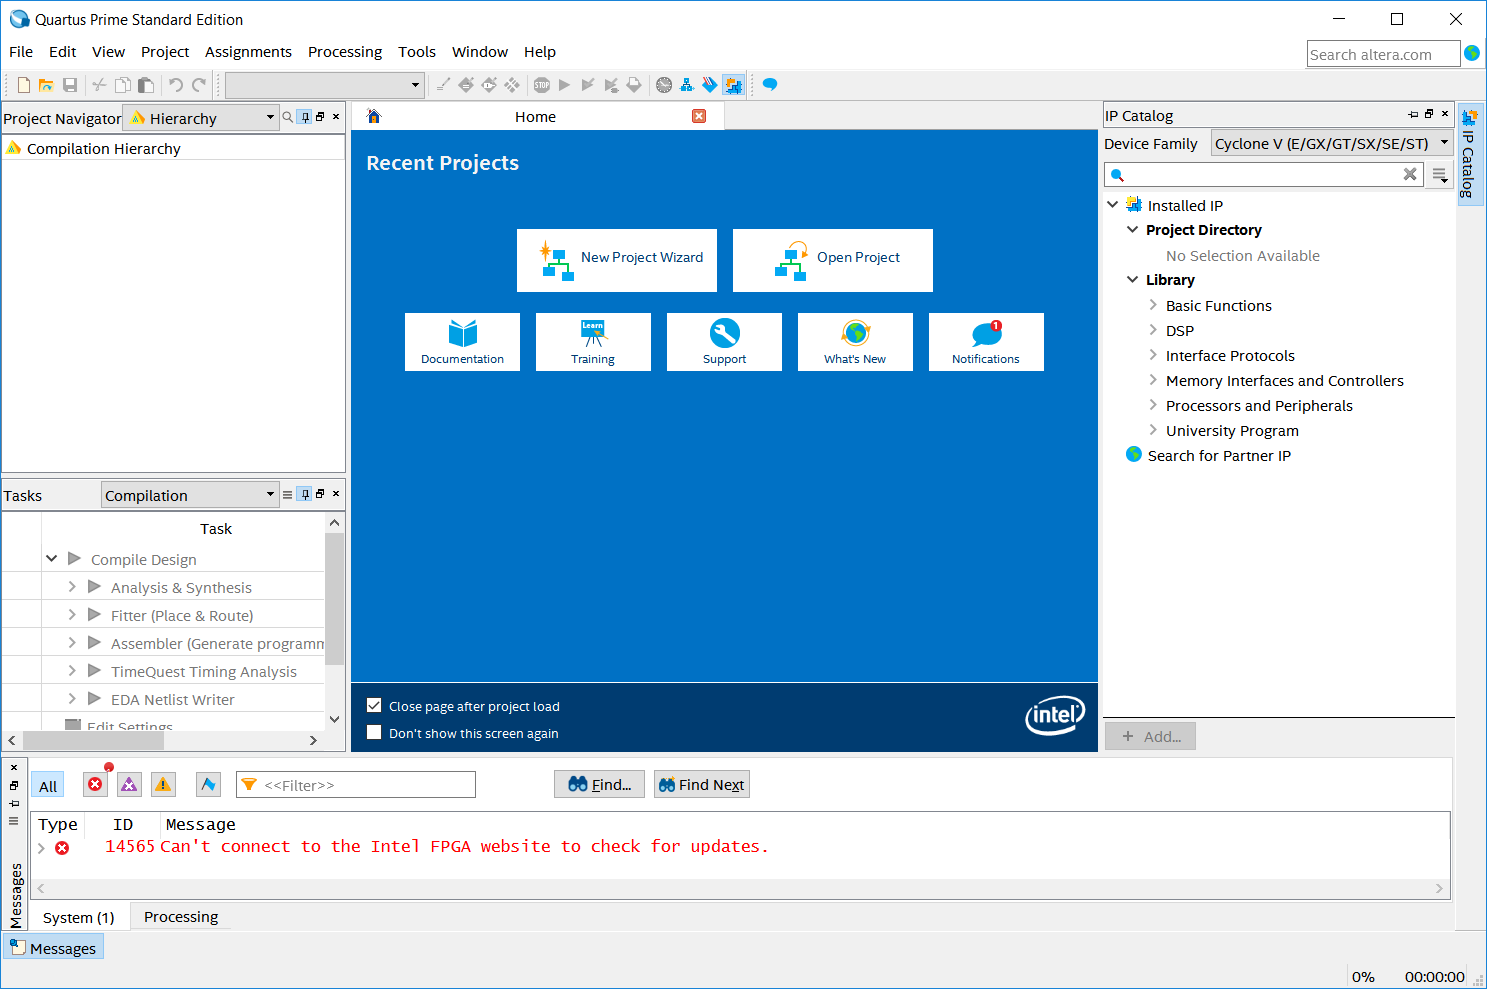
\includegraphics[scale=0.4]{figures/figure2.png}
   \caption{The main Quartus Prime display.} 
	 \label{fig:2}
	 \end{center}
\end{figure}

\begin{figure}[H]
   \begin{center}
      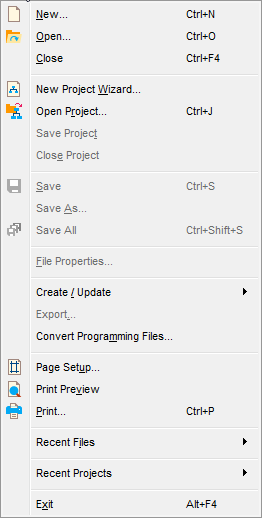
\includegraphics[scale=0.45]{figures/figure3.png}
   \caption{An example of the File menu.} 
	 \label{fig:3}
	 \end{center}
\end{figure}

\newpage
For some commands it is necessary to access two or more menus in sequence.
We use the convention {\sf Menu1 $>$ Menu2 $>$ Item} to indicate that 
to select the desired command 
the user should first click the left mouse button on {\sf Menu1}, then 
within this menu click on {\sf Menu2}, and then
within {\sf Menu2} click on {\sf Item}. For example, 
{\sf File $>$ Exit} uses the mouse to exit from the system.
Many commands can be invoked by clicking on an icon displayed in 
one of the toolbars. To see the command associated with an icon, position the mouse
over the icon and the command name will be shown in the status bar at the bottom of the screen.

%%%%%%%%%%%%%%%%%%%%%%%%%

%%%%%%%%%%%%%%%%%%%%%%%%%
% Quartus Online Help
\subsection{Quartus\textsuperscript{\textregistered} Prime Online Help}


Quartus Prime software provides comprehensive online documentation that answers
many of the questions that may arise when using the software. The documentation is accessed
from the {\sf Help} menu.
To get some idea of the extent of documentation provided,
it is worthwhile for the reader to browse through the {\sf Help}
menu.

The user can quickly search through the Help topics by using the 
search box in the top right corner of the main Quartus display.
Another method, context-sensitive help, is provided for quickly finding documentation for
specific topics. While using most applications, pressing the {\sf F1} function
key on the keyboard opens a Help display that
shows the commands available for the application. 

%%%%%%%%%%%%%%%%%%%%%%%%%

%%%%%%%%%%%%%%%%%%%%%%%%%
% Starting A New Project
\section{Starting a New Project}


To start working on a new design we first have to define a new 
{\it design project}.
Quartus Prime software makes the designer's task easy by providing support in the form
of a {\it wizard}.
Create a new project as follows:
\begin{enumerate}
\item Select {\sf File $>$ New Project Wizard} and click {\sf Next} to 
reach the window in Figure~\ref{fig:4},
which asks for the name and directory of the project.

\item Set the working directory to be {\it introtutorial};
of course, you can use some other directory name of your choice if you prefer.
The project must have a name, which is usually the same as the 
top-level design entity that will be included in the project.
Choose {\it light} as the name for both the project
and the top-level entity, as shown in Figure~\ref{fig:4}.  Press {\sf Next}. 
Since we have not yet created the directory {\it introtutorial},
Quartus Prime software displays the pop-up box in Figure~\ref{fig:5} asking if it should create
the desired directory. Click {\sf Yes}, which leads to
the window in Figure~\ref{fig:5_1}.

\begin{figure}[H]
   \begin{center}
      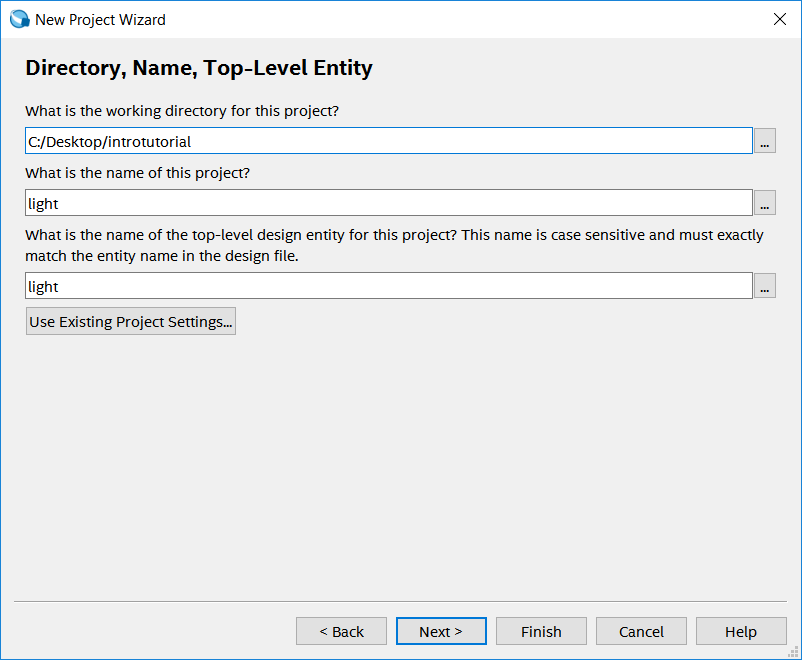
\includegraphics[scale=0.55]{figures/figure4.png}
   \caption{Creation of a new project.}
	 \label{fig:4}
	 \end{center}
\end{figure}

\begin{figure}[H]
   \begin{center}
      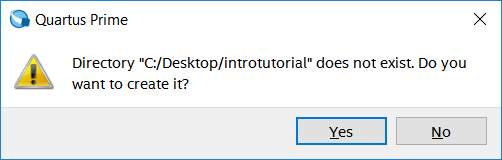
\includegraphics[scale=0.55]{figures/figure5.png}
   \caption{Quartus Prime software can create a new directory for the project.} 
	 \label{fig:5}
	 \end{center}
\end{figure}

\begin{figure}[H]
   \begin{center}
      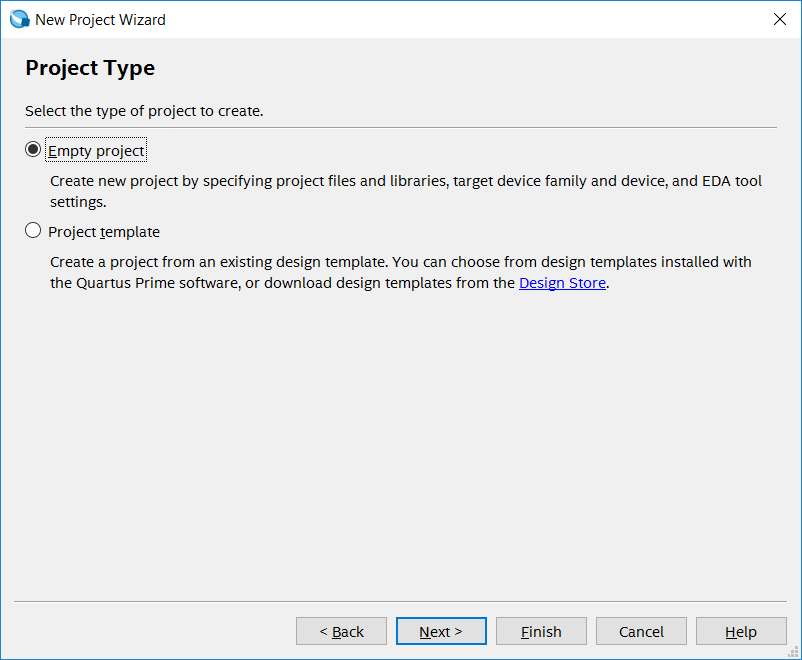
\includegraphics[scale=0.55]{figures/figure5_1.png}
   \caption{Choosing the project type.} 
	 \label{fig:5_1}
	 \end{center}
\end{figure}

\item The {\sf Project Type} window, shown in Figure~\ref{fig:5_1}, allows you to choose from
the {\sf Empty project} and the {\sf Project template} options. For this tutorial, choose {\sf Empty project} 
as we will be creating a project from scratch, and press {\sf Next} which leads to the window in Figure~\ref{fig:6}. 

\begin{figure}[H]
   \begin{center}
      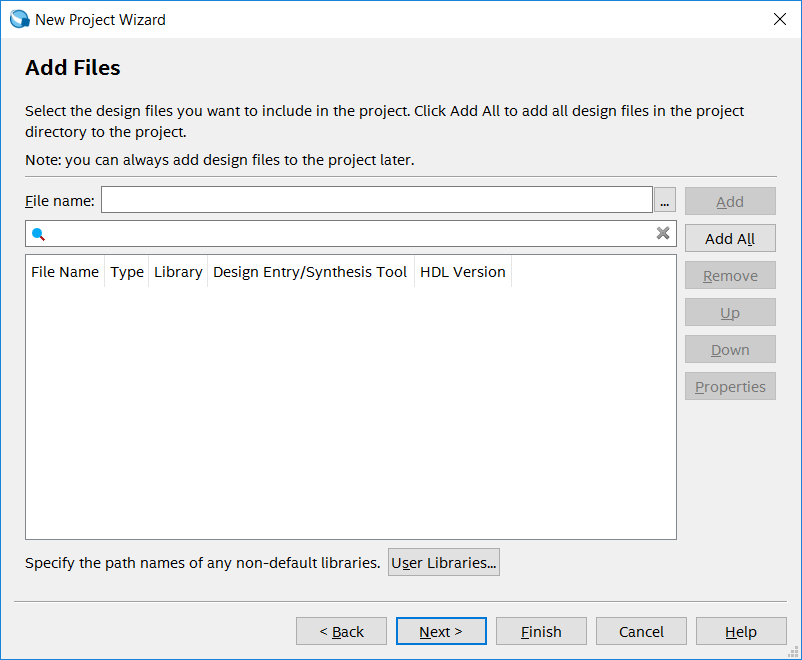
\includegraphics[scale=0.55]{figures/figure6.png}
   \caption{The wizard can include user-specified design files.} 
	 \label{fig:6}
	 \end{center}
\end{figure}

\item The wizard makes it easy to 
specify which existing files (if any) should be included in the project.
Assuming that we do not have any existing files, click {\sf Next}, which leads
to the window in Figure~\ref{fig:7}.

\begin{figure}[H]
   \begin{center}
      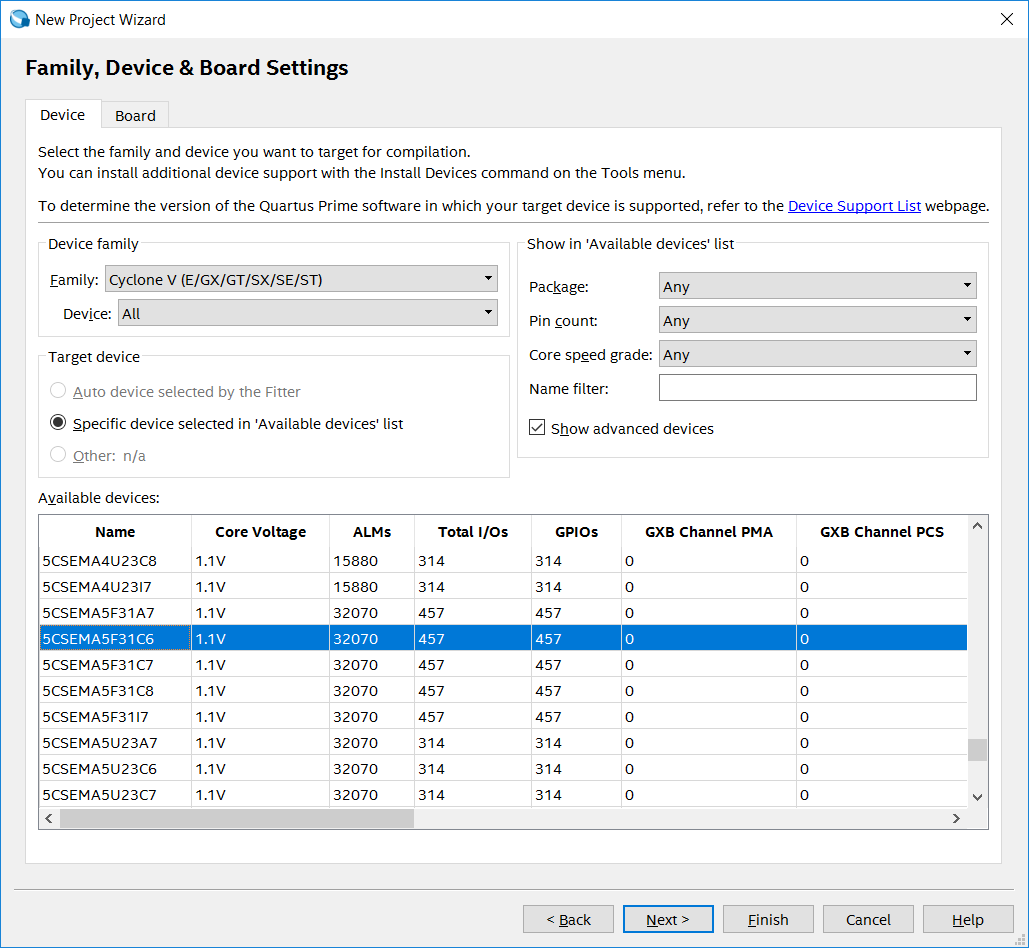
\includegraphics[scale=0.55]{figures/figure7.png}
   \caption{Choose the device family and a specific device.} 
	 \label{fig:7}
	 \end{center}
\end{figure}

\item We have to specify the type of device in which the designed circuit will 
be implemented.
Choose the Cyclone\textsuperscript{\textregistered} series device family for your DE-series board. 
We can let Quartus Prime software select a specific device in the family, 
or we can choose the device explicitly. 
We will take the latter approach. 
From the list of available devices, choose the appropriate device name for your DE-series board. A list of devices names on DE-series boards can be found in Table \ref{tab:device}. 
Press {\sf Next}, which opens the window in Figure~\ref{fig:8}.
 
\begin{table}[H]
	\begin{center}
	\begin{tabular}{| c | c |}
	\hline
	Board & Device Name \\
	\hline
	DE0-CV & Cyclone V 5CEBA4F23C7 \\
	\hline
	DE0-Nano & Cyclone IVE EP4CE22F17C6 \\
	\hline
	DE0-Nano-SoC & Cyclone V SoC 5CSEMA4U23C6\\
	\hline
	DE1-SoC & Cyclone V SoC 5CSEMA5F31C6 \\
	\hline
	DE2-115 & Cyclone IVE EP4CE115F29C7 \\
	\hline
	DE10-Lite & Max 10 10M50DAF484C7G \\
	\hline
	DE10-Standard & Cyclone V SoC 5CSXFC6D6F31C6 \\
	\hline
	DE10-Nano & Cyclone V SE 5CSEBA6U2317 \\
	\hline
	\end{tabular}
	\caption{DE-series FPGA device names}
	\label{tab:device}
	\end{center}
\end{table}

\begin{figure}[H]
   \begin{center}
      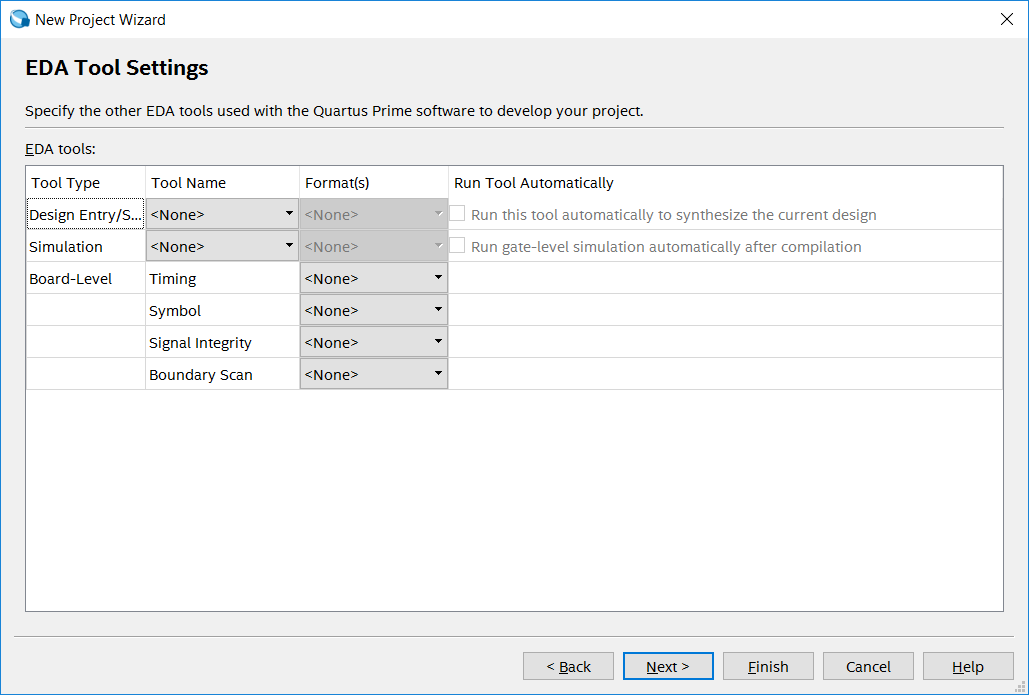
\includegraphics[scale=0.6]{figures/figure8.png}
   \caption{Other EDA tools can be specified.} 
	 \label{fig:8}
	 \end{center}
\end{figure}

\item The user can specify any third-party tools that should be used.
A commonly used term for CAD software for electronic circuits
is {\it EDA tools}, where the acronym stands for Electronic Design Automation.
This term is used in Quartus Prime messages that refer to third-party tools, 
which are the tools developed and marketed by companies other than Intel.
Since we will rely solely on Quartus Prime tools, we will not choose 
any other tools.  Press {\sf Next}.
 
\item A summary of the chosen settings appears in the screen shown in Figure~\ref{fig:9}.
Press {\sf Finish}, which returns to the main Quartus Prime window, 
but with {\it light} specified as the new project,
in the title bar, as indicated in Figure~\ref{fig:10}.
\end{enumerate}

\begin{figure}[H]
   \begin{center}
      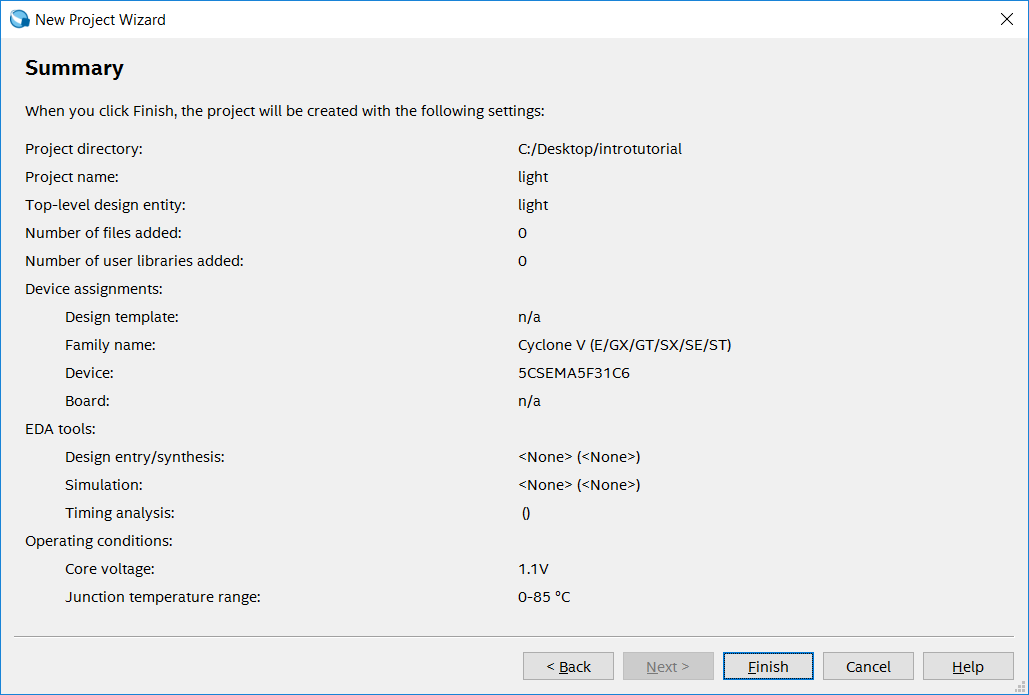
\includegraphics[scale=0.5]{figures/figure9.png}
   \caption{Summary of project settings.} 
	 \label{fig:9}
	 \end{center}
\end{figure}

\begin{figure}[H]
   \begin{center}
      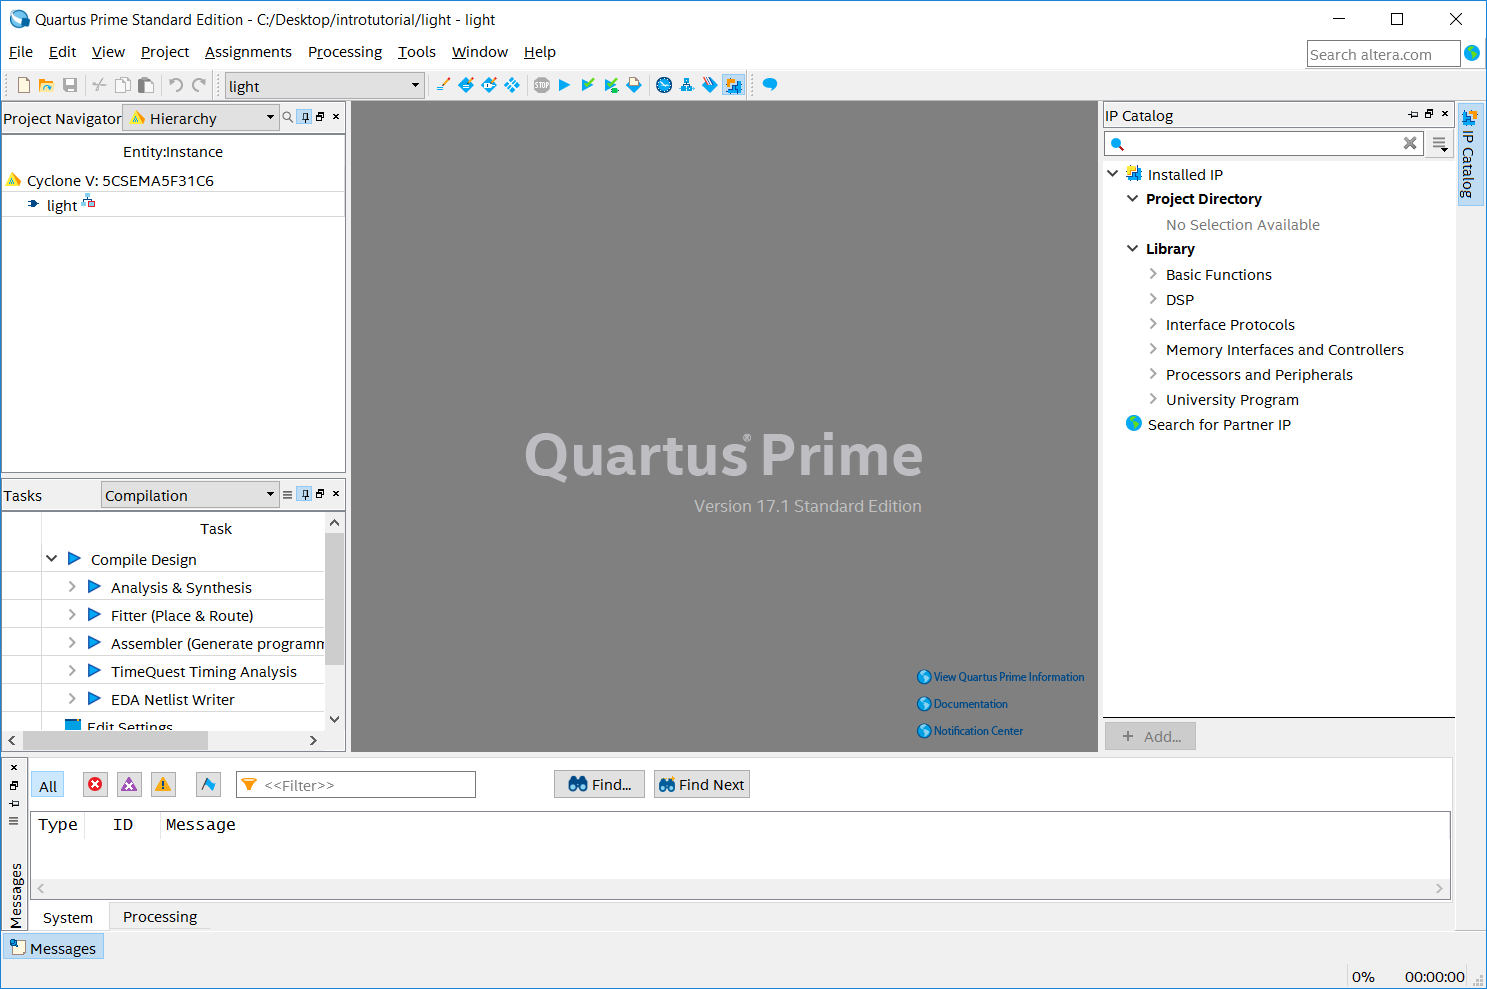
\includegraphics[scale=0.4]{figures/figure10.png}
   \caption{The Quartus Prime window for a created project.} 
	 \label{fig:10}
	 \end{center}
\end{figure}

%%%%%%%%%%%%%%%%%%%%%%%%%

%%%%%%%%%%%%%%%%%%%%%%%%%
% Design Entry Using VHDL
\section{Design Entry Using Verilog Code}


\noindent
As a design example, we will use the two-way light controller circuit shown in 
Figure~\ref{fig:11}. The circuit can be used to control a single light from either of the
two switches, $x_1$ and $x_2$, where a closed switch corresponds to the logic value 1.
The truth table for the circuit is also given in the figure. Note that
this is just the Exclusive-OR function of the inputs $x_1$ and $x_2$,
but we will specify it using the gates shown.

\begin{figure}[H]
   \begin{center}
      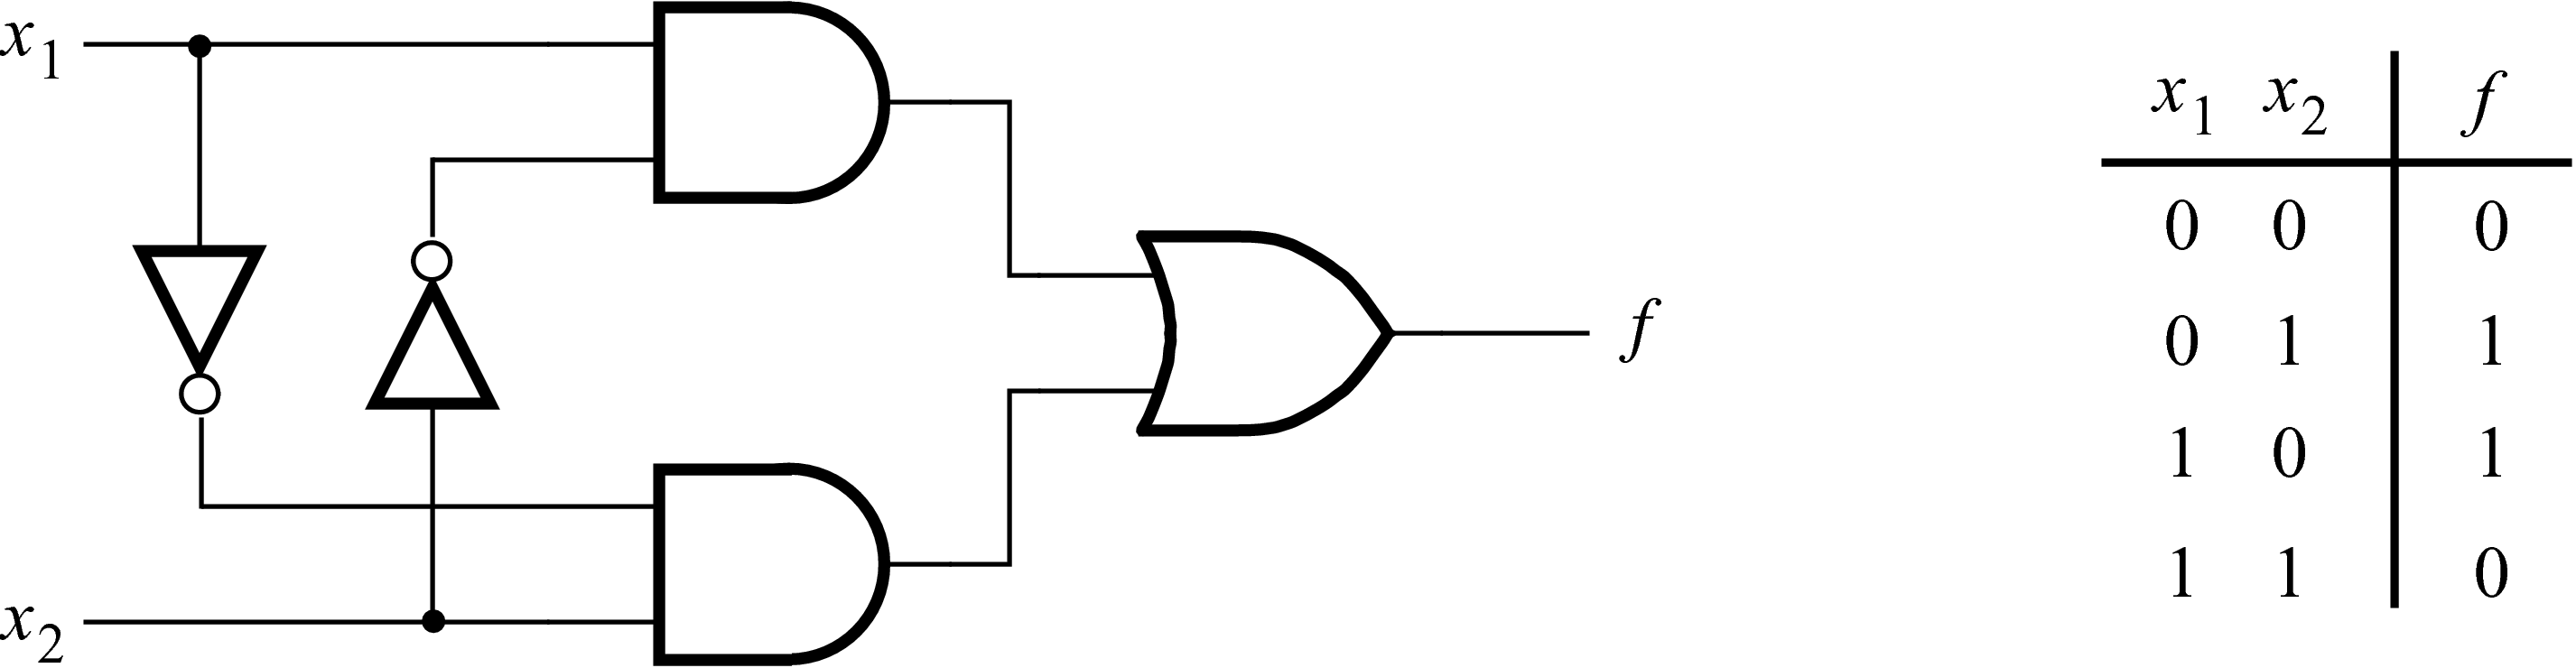
\includegraphics[scale=1]{figures/figure11.png}
   \caption{The light controller circuit.} 
	 \label{fig:11}
	 \end{center}
\end{figure}

The required circuit is described by the Verilog code in Figure~\ref{fig:12}.
Note that the Verilog module is called {\it light} to match the name given in 
Figure~\ref{fig:4}, which was specified when the project was created.
This code can be typed into a file by using any text editor
that stores ASCII files, or by using the Quartus Prime text editing facilities.
While the file can be given any name, it is a common designers' practice to
use the same name as the name of the top-level Verilog module.
The file name must include the extension $v$, which indicates a Verilog
file. So, we will use the name {\it light.v}.

\lstset{language=Verilog}
\begin{figure}[H]
\begin{center}
\begin{lstlisting}
module light (x1, x2, f);
	input x1, x2;
	output f;
	assign f = (x1 & ~x2)|(~x1 & x2);
endmodule 
\end{lstlisting}
\end{center}
\vspace{-0.33in}
	\caption{Verilog code for the circuit in Figure 11.}
	\label{fig:12}
\end{figure}

\subsection{Using the Quartus\textsuperscript{\textregistered}	 Prime Text Editor}

\noindent 
This section shows how to use the Quartus Prime Text Editor.
You can skip this section if you prefer to use some other text editor
to create the Verilog source code file, which we will name {\it light.v}. 

Select {\sf File $>$ New} to get the window in Figure~\ref{fig:13}, 
choose {\sf Verilog HDL File}, and click {\sf OK}. 
This opens the Text Editor window. 
The first step is to specify a name
for the file that will be created. Select {\sf File $>$ Save As}
to open the pop-up box depicted in Figure~\ref{fig:14}. 
In the box labeled {\sf Save as type} choose {\sf Verilog HDL File}.
In the box labeled {\sf File name} type {\it light}.
Put a checkmark in the box {\sf Add file to current project}.
Click {\sf Save}, which puts the file into the directory
{\it introtutorial} and leads to the Text Editor window shown
in Figure~\ref{fig:15}. 
Enter the Verilog code in Figure~\ref{fig:12}
into the Text Editor and save the file by typing {\sf File $>$ Save}, or by typing 
the shortcut {\sf Ctrl-s}.

Most of the commands available in the Text Editor are self-explanatory. 
Text is entered at the {\it insertion point}, which is indicated by a thin
vertical line. The insertion point can be moved either by using the
keyboard arrow keys or by using the mouse. Two features of 
the Text Editor are especially convenient for typing Verilog
code. First, the editor can display different types of Verilog
statements in different colors, which is the default choice. 
Second, the editor can automatically
indent the text on a new line so that it matches the previous line. 
Such options can be controlled by the settings 
in {\sf Tools $>$ Options $>$ Text Editor}.

\begin{figure}[H]
   \begin{center}
      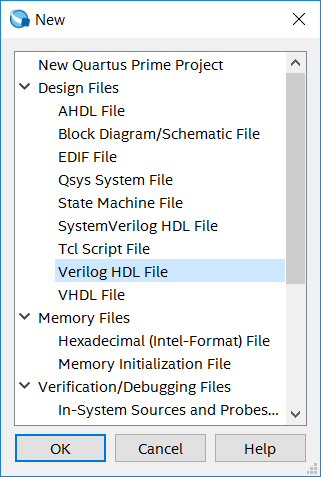
\includegraphics[scale=0.65]{figures/figure13.png}
   \caption{Choose to prepare a Verilog file.} 
	 \label{fig:13}
	 \end{center}
\end{figure}

\begin{figure}[H]
   \begin{center}
      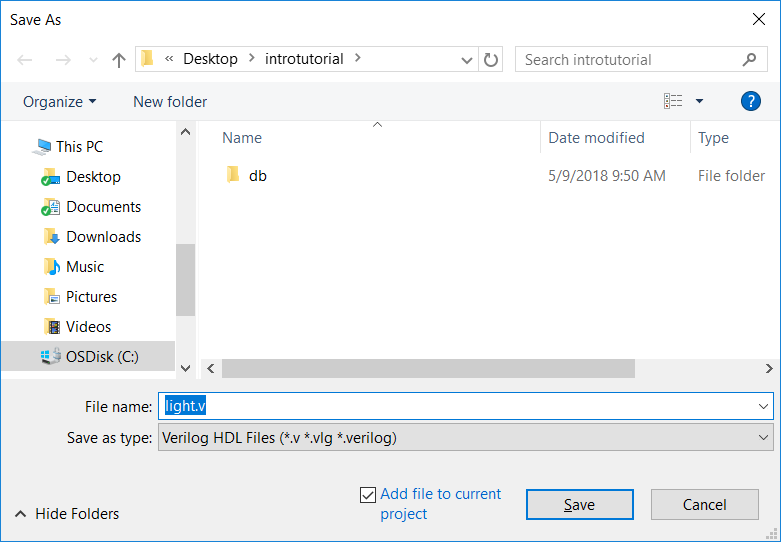
\includegraphics[scale=0.55]{figures/figure14.png}
   \caption{Name the file.} 
	 \label{fig:14}
	 \end{center}
\end{figure}

\begin{figure}[H]
   \begin{center}
      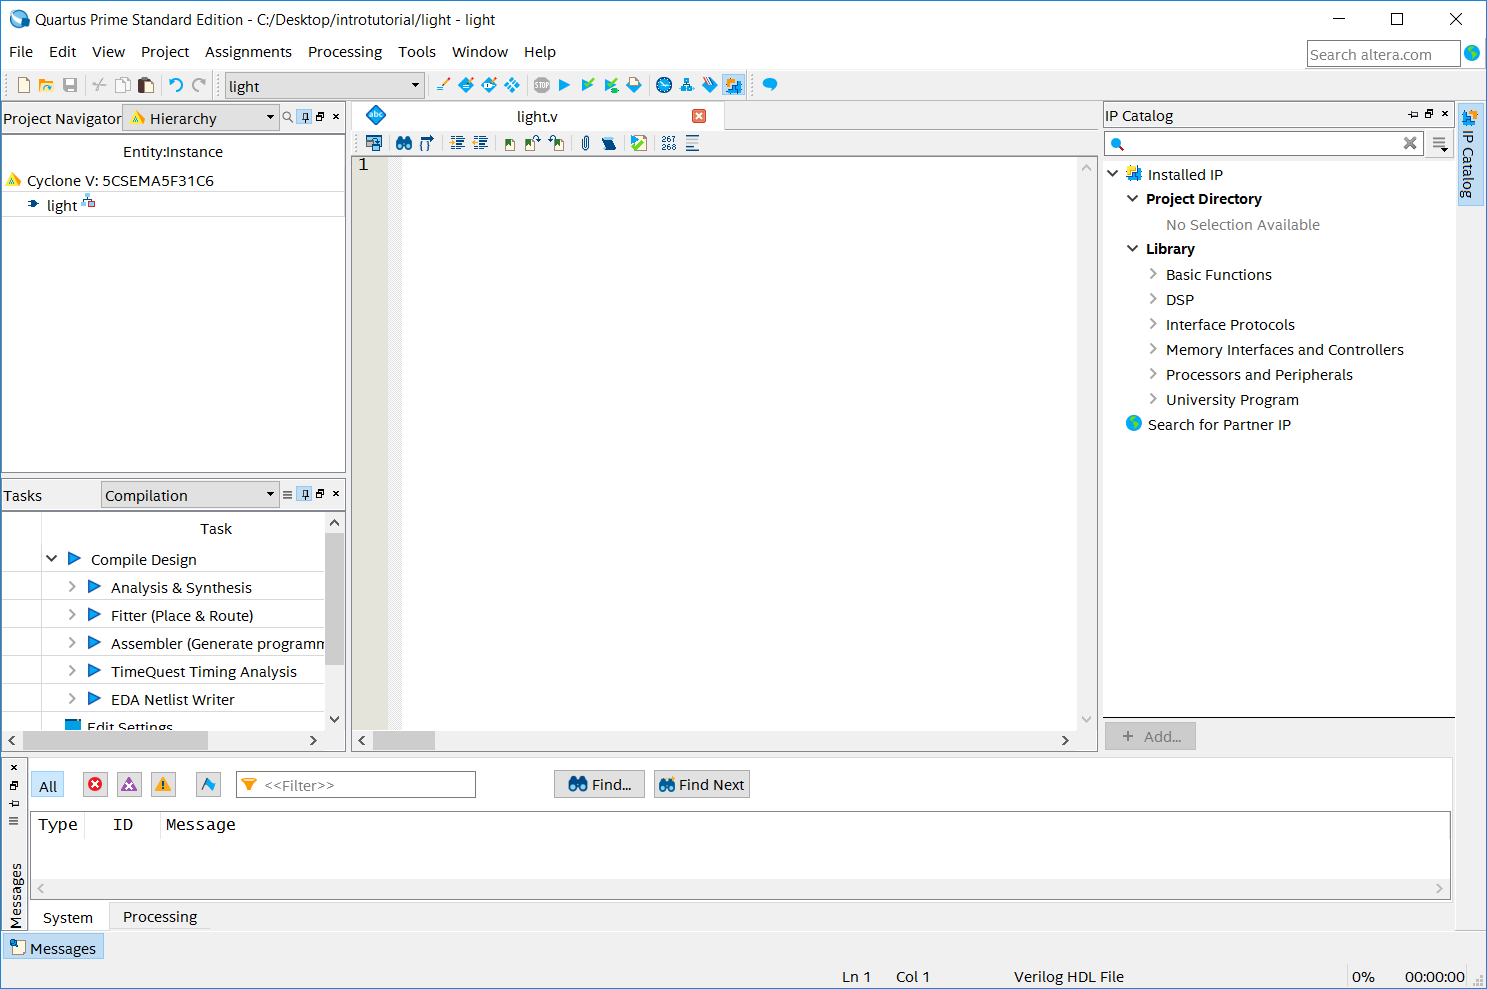
\includegraphics[scale=0.40]{figures/figure15.png}
   \caption{Text Editor window.} 
	 \label{fig:15}
	 \end{center}
\end{figure}

\subsubsection{Using Verilog Templates}

The syntax of Verilog code is sometimes difficult for a
designer to remember. To help with this issue, the Text Editor
provides a collection of {\it Verilog templates}. The templates provide
examples of various types of Verilog statements, such as a {\bf module}
declaration, an {\bf always} block, and assignment statements. 
It is worthwhile to browse through the templates
by selecting {\sf Edit $>$ Insert Template $>$ Verilog HDL} to become 
familiar with this resource.

\subsection{Adding Design Files to a Project}

As we indicated when discussing Figure~\ref{fig:6}, you can tell Quartus Prime software
which design files it should use as part of the current project.
To see the list of files already included in the {\it light} project,
select {\sf Assignments $>$ Settings}, which leads to the window in Figure~\ref{fig:16}.
As indicated on the left side of the figure, click on the item {\sf Files}.
An alternative way of making this selection is to choose
{\sf Project $>$ Add/Remove Files in Project}.

If you used the Quartus Prime Text Editor to create the file and checked
the box labeled {\sf Add file to current project},
as described in Section 5.1, then the {\it light.v}
file is already a part of the project and will be listed in
the window in Figure~\ref{fig:16}.
Otherwise, the file must be added to the project. 
So, if you did not use the Quartus Prime Text Editor, then place a copy of the 
file {\it light.v}, which you created using some other text editor, into 
the directory {\it introtutorial}.
To add this file to the project, click on the {\sf ...} button next to the 
box labeled {\sf File name} in
Figure~\ref{fig:16} to get the pop-up window in Figure~\ref{fig:17}.
Select the {\it light.v} file and click {\sf Open}.
The selected file is now indicated in the {\sf File name} box in Figure~\ref{fig:16}. 
Click {\sf Add} then {\sf OK} to include the {\it light.v} file in the project.
We should mention that in many cases the Quartus Prime software is able to 
automatically find the right files to use for each entity 
referenced in Verilog code, even if the file has not been 
explicitly added to the project. However, for complex projects that
involve many files it is a good design practice to specifically
add the needed files to the project, as described above.

\begin{figure}[H]
   \begin{center}
      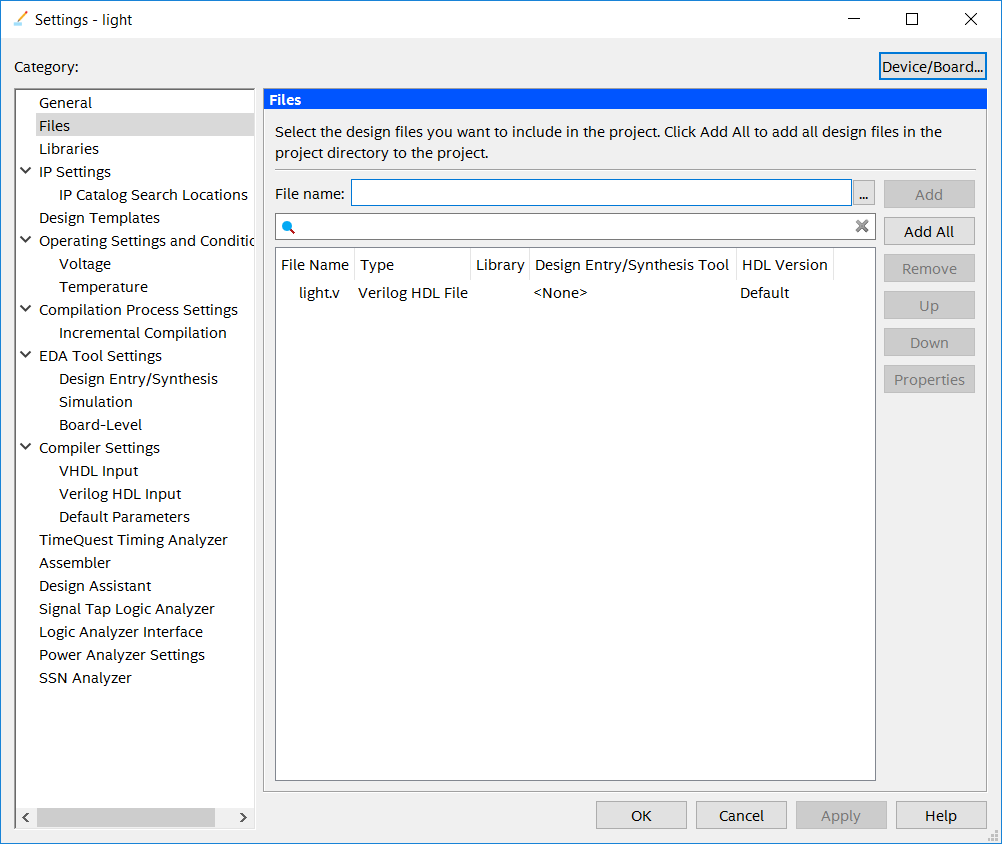
\includegraphics[scale=0.55]{figures/figure16.png}
   \caption{Settings window.} 
	 \label{fig:16}
	 \end{center}
\end{figure}

\begin{figure}[H]
   \begin{center}
      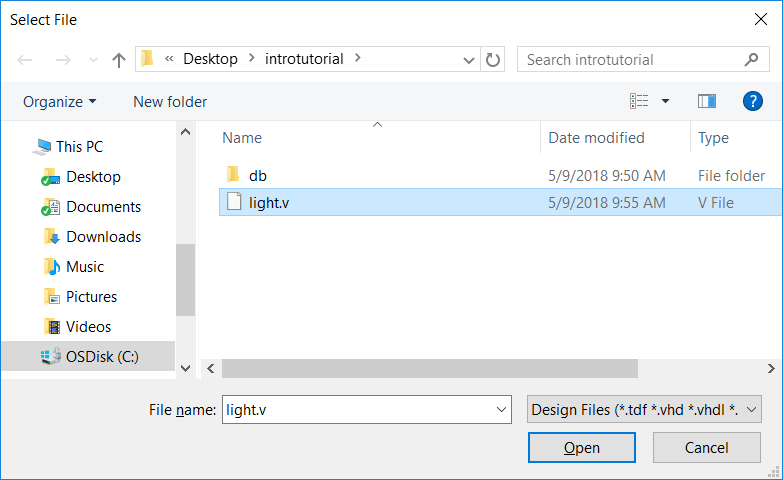
\includegraphics[scale=0.65]{figures/figure17.png}
   \caption{Select the file.} 
	 \label{fig:17}
	 \end{center}
\end{figure}

%%%%%%%%%%%%%%%%%%%%%%%%%

%%%%%%%%%%%%%%%%%%%%%%%%%
% Compiling Designed Circuit
\section{Compiling the Designed Circuit}


The Verilog code in the file {\it light.v} is processed by several 
Quartus Prime tools that analyze the code, synthesize the circuit,
and generate an implementation of it for the target chip. 
These tools are controlled by the application program called the {\it Compiler}.

Run the Compiler by selecting {\sf Processing $>$ Start Compilation}, or by 
clicking on the toolbar icon 
\includegraphics[scale=0.45]{figures/icon5.png} that looks like a
blue triangle. Your project must be saved before compiling. 
As the compilation moves through various stages, its progress is reported
in a window on the left side of the Quartus Prime display.
In the message window, at the bottom of the figure, various messages are displayed
throughout the compilation process.
In case of errors, there will be appropriate messages given.

When the compilation is finished, a compilation report is produced.
A tab showing this report is opened automatically, as seen in Figure~\ref{fig:20}.
The tab can be closed in the normal way, and it can be opened at any time
either by selecting {\sf Processing $>$ Compilation Report} or by clicking on 
the icon 
\includegraphics[scale=0.45]{figures/icon6.png}.
The report includes a number of sections listed on the left side.
Figure~\ref{fig:20} displays the Compiler Flow Summary section, which
indicates that only one logic element and three pins are needed to implement this 
tiny circuit on the selected FPGA chip.

\begin{figure}[H]
   \begin{center}
      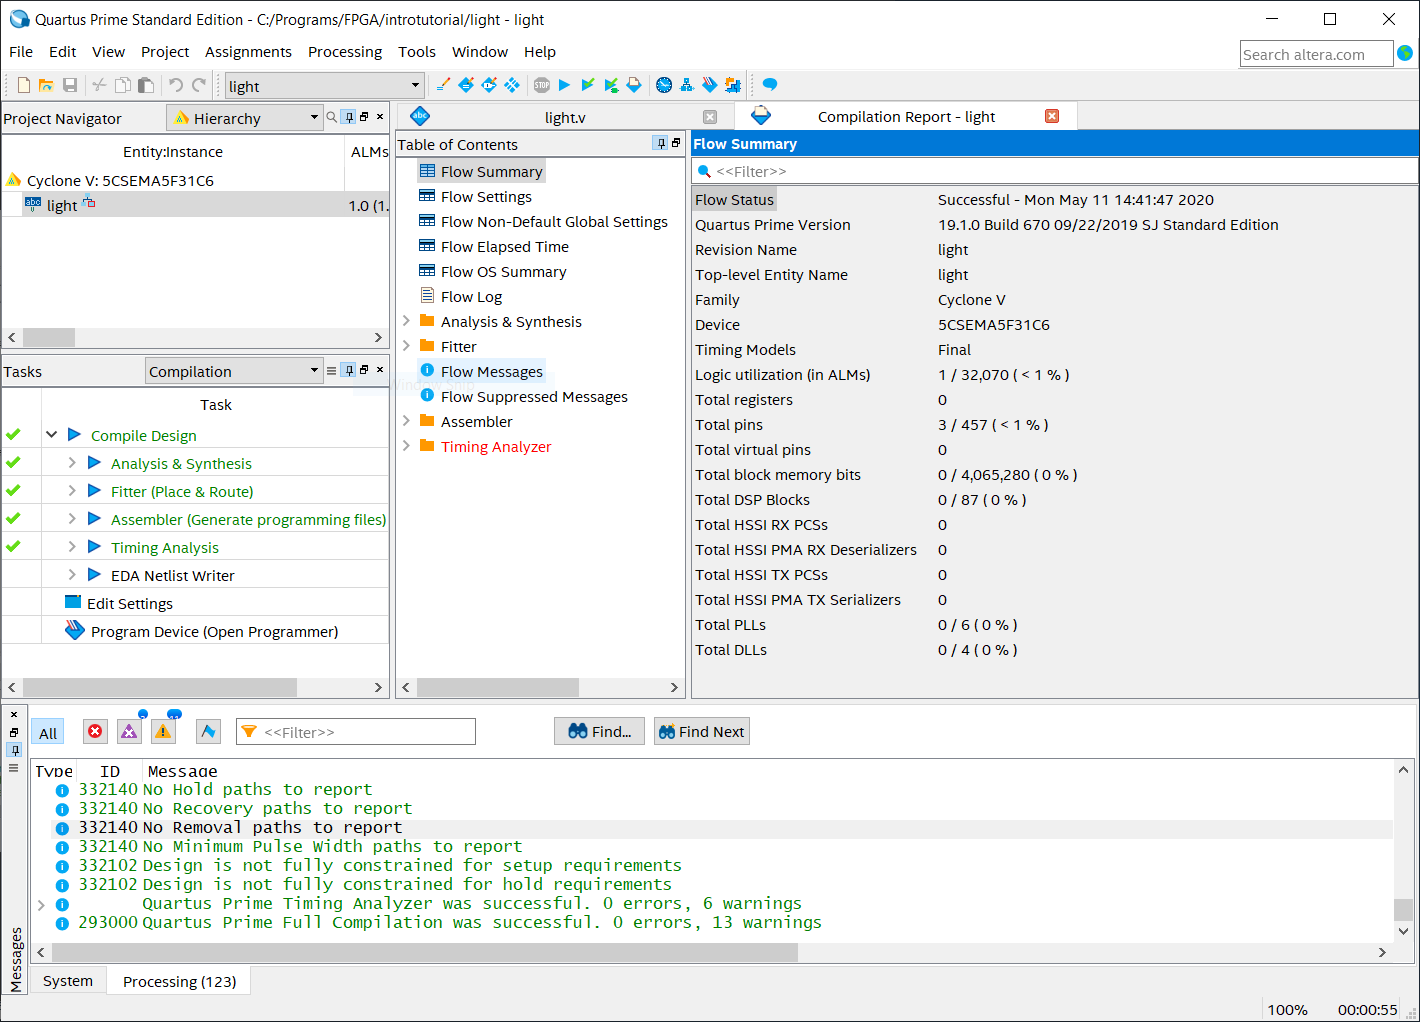
\includegraphics[scale=0.5]{figures/figure18.png}
   \caption{Display after a successful compilation.} 
	 \label{fig:18}
	 \end{center}
\end{figure}

\subsection{Errors}

Quartus Prime software displays messages produced during compilation in the Messages window.
If the Verilog design file is correct, one of the messages will
state that the compilation was successful and that there are no
errors.

If the Compiler does not report zero errors, then there is at least one mistake 
in the Verilog code. In this case a
message corresponding to each error found will
be displayed in the Messages window.
Double-clicking on an error message will highlight the offending
statement in the Verilog code in the Text Editor window. 
Similarly, the Compiler may display some warning messages. Their details can be
explored in the same way as in the case of error messages.
The user can obtain more information about a specific error or warning message
by selecting the message and pressing the {\sf F1} function key.

To see the effect of an error, open the file {\it light.v}.
Remove the semicolon in the {\bf assign} statement, illustrating a
typographical error that is easily made.
Compile the erroneous design file by clicking on the 
\includegraphics[scale=.45]{figures/icon5.png} icon.
A pop-up box will ask if the changes made to the {\it light.v} file should be saved;
click {\sf Yes}. After trying to compile the circuit,
Quartus Prime software will display error messages in the Messages window, and 
show that the compilation failed in the {\sf Analysis \& Synthesis} stage of the compilation process.
The compilation report summary, given in Figure~\ref{fig:19}, 
confirms the failed result. In the Table of Contents panel, expand the {\sf Analysis \& Synthesis} part of the report
and then select {\sf Messages} to have the messages displayed as shown in Figure~\ref{fig:20}.
The Compilation Report can be displayed as a separate window as in Figure~\ref{fig:20} 
by right-clicking its tab and selecting {\sf Detach Window}, and can be reattached by clicking
{\sf Window > Attach Window}. Double-click on the first error message. 
Quartus Prime software responds by opening the {\it light.v}
file and highlighting the statement which is affected by the error,
as shown in Figure~\ref{fig:21}.
Correct the error and recompile the design.

\begin{figure}[H]
   \begin{center}
      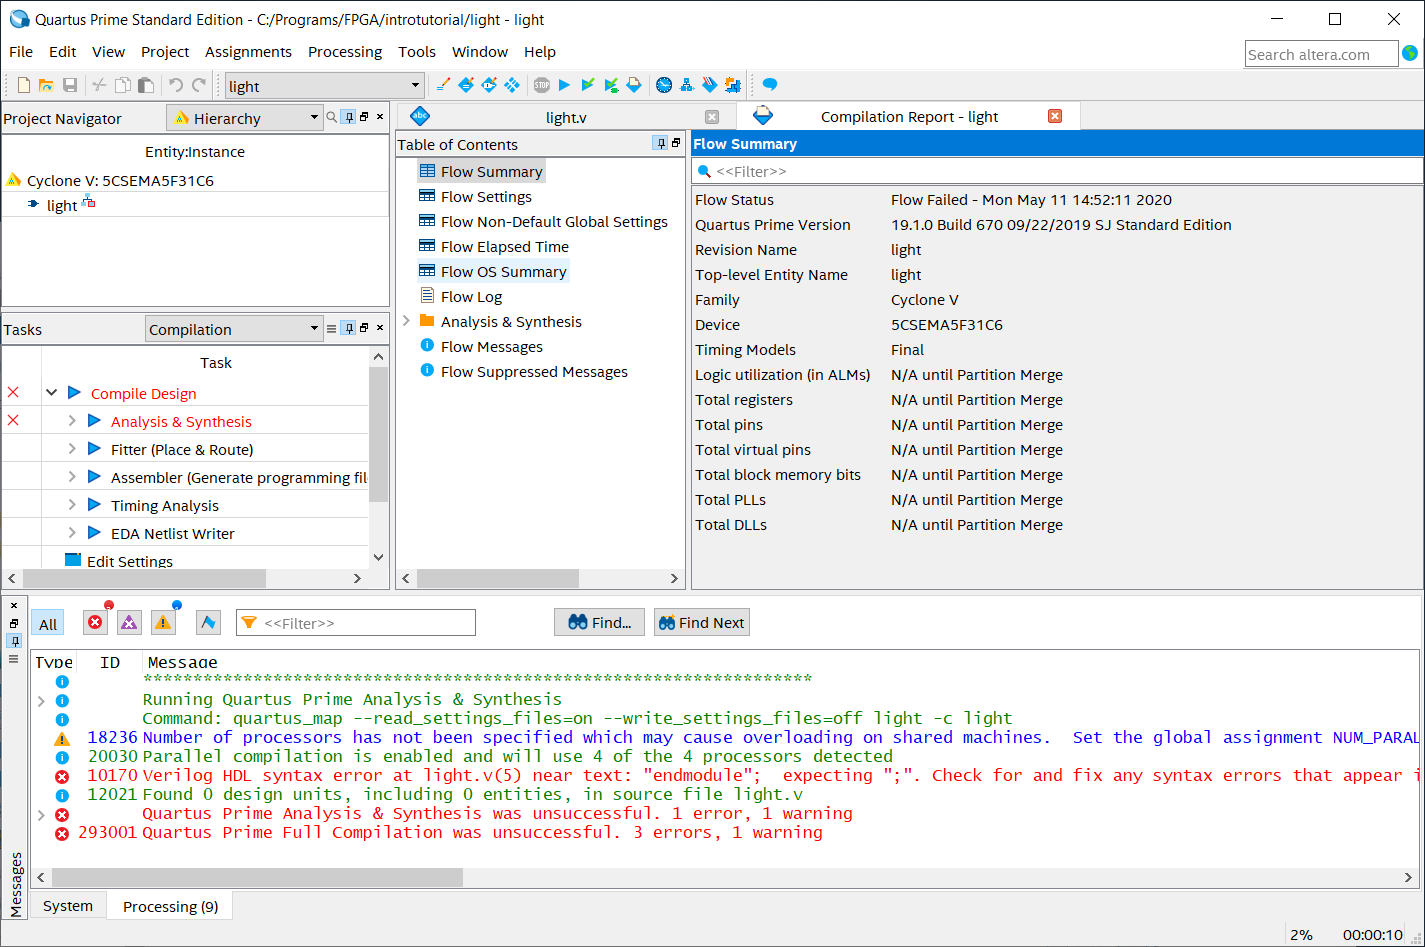
\includegraphics[scale=0.5]{figures/figure19.png}
   \caption{Compilation report for the failed design.} 
	 \label{fig:19}
	 \end{center}
\end{figure}

\begin{figure}[H]
   \begin{center}
      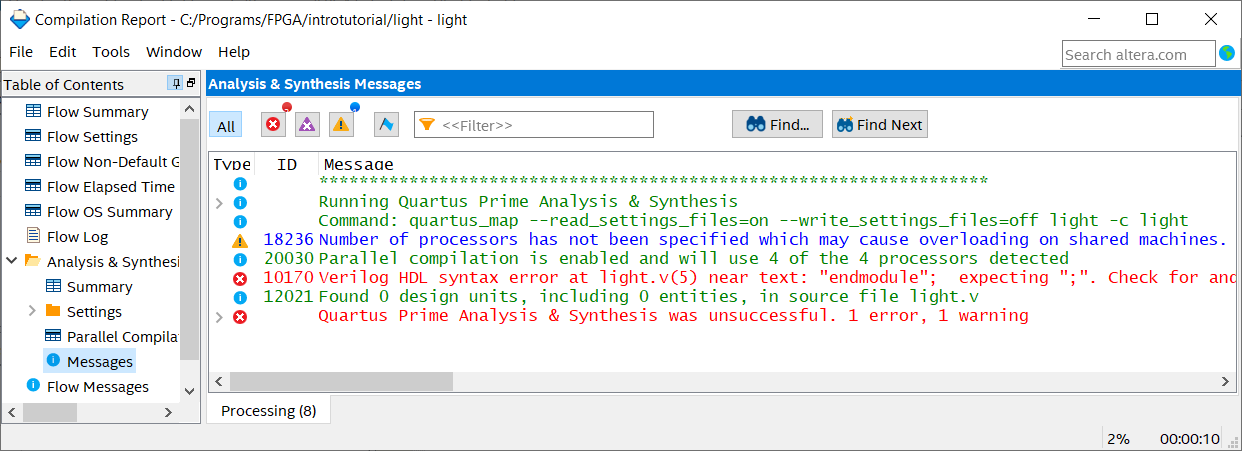
\includegraphics[scale=0.5]{figures/figure20.png}
   \caption{Error messages.}
	 \label{fig:20}
	 \end{center}
\end{figure}

\begin{figure}[H]
   \begin{center}
      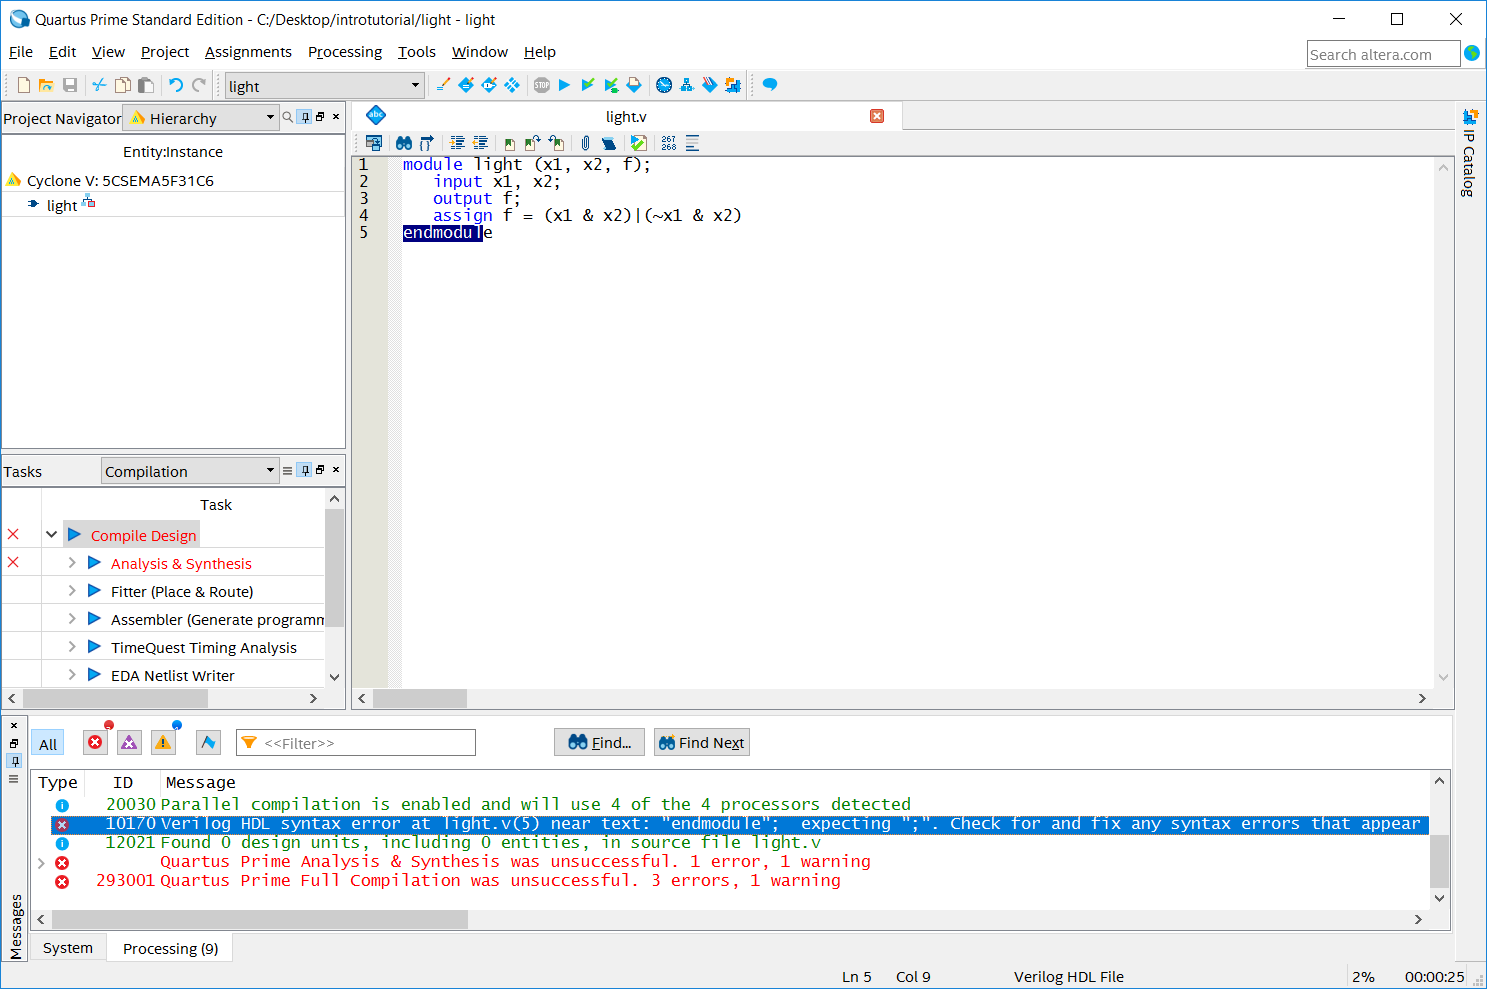
\includegraphics[scale=0.40]{figures/figure21.png}
   \caption{Identifying the location of the error.} 
	 \label{fig:21}
	 \end{center}
\end{figure}

%%%%%%%%%%%%%%%%%%%%%%%%%

%%%%%%%%%%%%%%%%%%%%%%%%%
% Pin Assignments
\section{Pin Assignment}


During the compilation above, the Quartus Prime Compiler was free to choose any
pins on the selected FPGA to serve as inputs and outputs. However, the DE-series board
has hardwired connections between the FPGA pins and the other components on the board.
We will use two toggle switches, labeled $SW_0$ and $SW_1$, to provide the
external inputs, $x_1$ and $x_2$, to our example circuit. These switches are connected
to the FPGA pins listed in Table \ref{tab:pinassign}. We will connect the output $f$ to a
light-emitting diode on your DE-series board. For the DE2-115 we will use a green LED: $LEDG_0$.
On the DE0-CV, DE1-SoC, DE-10 Lite and DE10-Standard we will use $LEDR_0$. On the DE0-Nano and DE0-Nano-SoC, we will use $LED_0$
The FPGA pin assignment for the LEDs can also be found in Table~\ref{tab:pinassign}.

\begin{table}[H]
\centering
\begin{tabular}{| c | c | c | c |}
\hline
Component & $SW_0$ & $SW_1$ & {\it LEDG}$_0$, {\it LED}$_0$, or {\it LEDR}$_0$ \\
\hline
DE0-CV & PIN$\_$U13 & PIN$\_$V13 & PIN$\_$AA2 \\
\hline
DE0-Nano & PIN$\_$M1 & PIN$\_$T8 & PIN$\_$A1 \\
\hline
DE0-Nano-SoC & PIN$\_$L10 & PIN$\_$L9 & PIN$\_$W15 \\
\hline
DE2-115 & PIN$\_$AB28 & PIN$\_$AC28 & PIN$\_$E21 \\
\hline
DE1-SoC & PIN$\_$AB12 & PIN$\_$AC12 & PIN$\_$V16 \\
\hline
DE10-Lite & PIN$\_$C10 & PIN$\_$C11 & PIN$\_$A8 \\
\hline
DE10-Standard & PIN$\_$AB30 & PIN$\_$AB28 & PIN$\_$AA24 \\
\hline
DE10-Nano & PIN$\_$Y24 & PIN$\_$W24 & PIN$\_$W15 \\
\hline
\end{tabular}
 
\caption{DE-Series Pin Assignments}
\label{tab:pinassign}
\end{table}

\begin{figure}[H]
   \begin{center}
      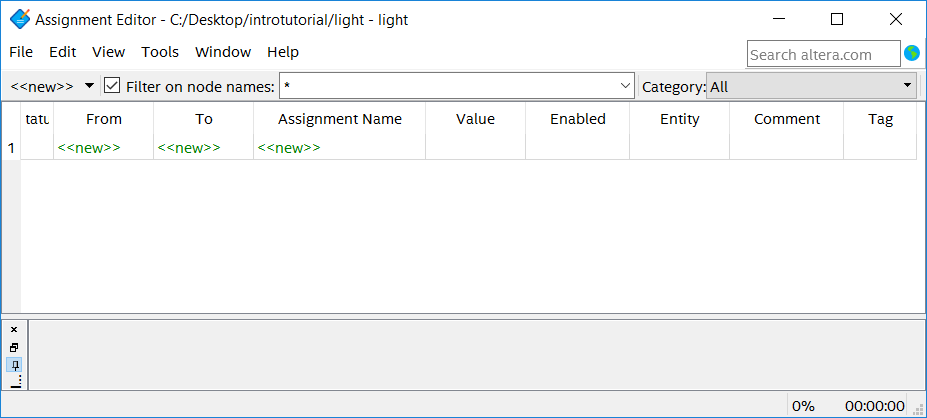
\includegraphics[scale=0.65]{figures/figure22.png}
   \caption{The Assignment Editor window.} 
	 \label{fig:22}
	 \end{center}
\end{figure}

Pin assignments are made by using the Assignment Editor. 
Select {\sf Assignments $>$ Assignment Editor} to reach the window in Figure~\ref{fig:22}
(shown here as a detached window).
In the {\sf Category} drop-down menu select {\sf All}. Click on the {\sf $<$$<$new$>$$>$} button
located near the top left corner to make a new item appear in the table. Double click the box
under the column labeled To so that the Node Finder button 
\includegraphics[scale=0.65]{figures/icon7.png}
appears. Click on the button (not the drop down arrow) to reach the window in Figure~\ref{fig:23}. Click on 
\includegraphics[scale=0.6]{figures/icon12.png} and 
\includegraphics[scale=0.6]{figures/icon15.png} to show or hide more search options.
In the {\sf Filter} drop-down menu select {\sf Pins: all}. Then click the {\sf List} button to display
the input and output pins to be assigned: $f$, $x1$, and $x2$.
Click on $x1$ as the first pin to be assigned and click the {\sf >} button; this will enter
$x1$ in the Selected Nodes box.  Click {\sf OK}. $x1$ will now appear in the box under the column
labeled To. Alternatively, the node name can be entered directly by double-clicking the box
under the To column and typing in the node name.

Follow this by double-clicking on the box to the right of this new $x1$ entry, in the column
labeled Assignment Name. Now, the drop-down menu in Figure~\ref{fig:24} appears. Scroll down and select 
{\sf Location (Accepts wildcards/groups)}. Instead of scrolling down the menu to find the desired item, 
you can just type the first letter of the item in the Assignment Name box. In this case the desired
item happens to be the first item beginning with L. Finally, double-click the box in the column labeled Value.
Type the pin assignment corresponding to $SW_0$ for your DE-series board, as listed in Table \ref{tab:pinassign}.

Use the same procedure to assign input $x2$ and output $f$ to the appropriate pins listed in
Table \ref{tab:pinassign}. An example using a DE1-SoC board is shown in Figure~\ref{fig:25}.
To save the assignments made, choose {\sf File $>$ Save}. You can also simply close 
the Assignment Editor window, in which case a pop-up box will ask if you want to save
the changes to assignments; click {\sf Yes}.
Recompile the circuit, so that it will be compiled with the correct pin assignments.


\begin{figure}[H]
   \begin{center}
      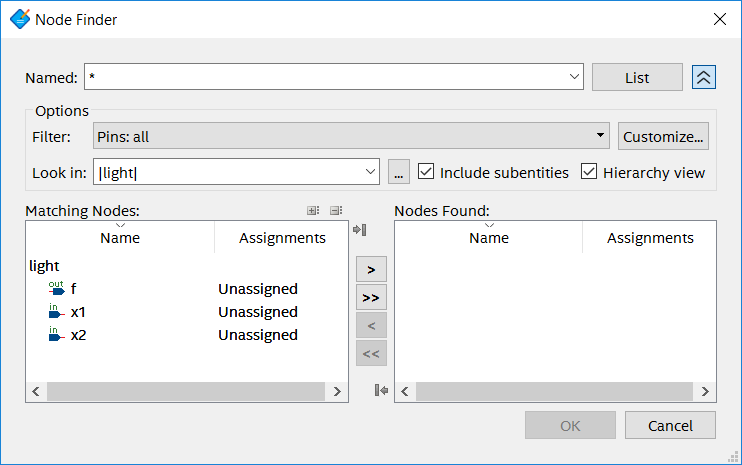
\includegraphics[scale=0.65]{figures/figure23.png}
   \caption{The Node Finder displays the input and output names.} 
	 \label{fig:23}
	 \end{center}
\end{figure}

\begin{figure}[H]
   \begin{center}
      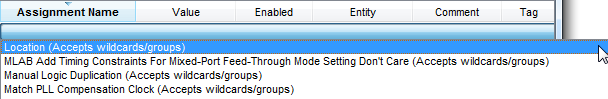
\includegraphics[scale=0.65]{figures/figure24.png}
   \caption{The available assignment names for a DE-series board.} 
	 \label{fig:24}
	 \end{center}
\end{figure}


\begin{figure}[H]
   \begin{center}
      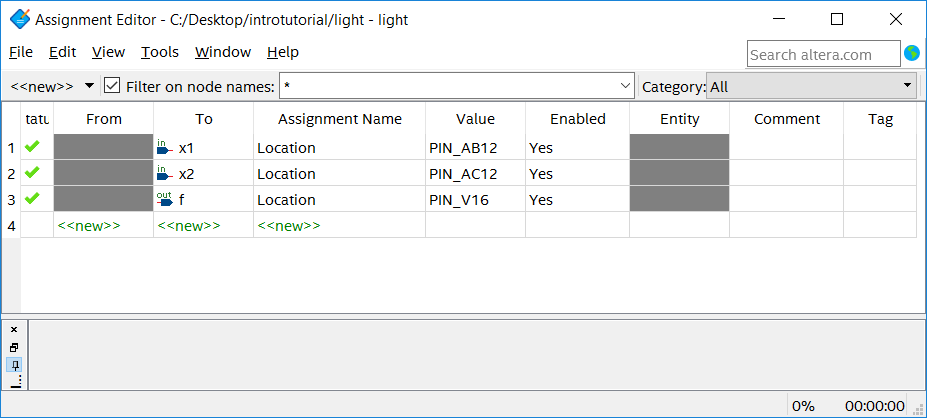
\includegraphics[scale=0.65]{figures/figure25.png}
   \caption{The complete assignment.} 
	 \label{fig:25}
	 \end{center}
\end{figure}

The DE-series board has fixed pin assignments. Having finished one design, the user will want
to use the same pin assignment for subsequent designs. Going through the procedure 
described above becomes tedious if there are many pins used in the design.
A useful Quartus Prime feature allows the user to both
export and import the pin assignments from a special file format, 
rather than creating them manually
using the Assignment Editor. A simple file format that can be used for this purpose
is the {\it Quartus Settings File (QSF)} format. The format for the file for our simple project (on a DE1-SoC board) is

\begin{center}
\begin{verbatim}
	set_location_assignment PIN_AB12 -to x1
	set_location_assignment PIN_AC12 -to x2
	set_location_assignment PIN_V16 -to f
\end{verbatim}
\end{center}

\noindent
By adding lines to the file, any number of pin assignments can be created.
Such {\it qsf} files can be imported into any design project.

If you created a pin assignment for a particular project, you can export it
for use in a different project. To see how this is done, open again the Assignment Editor
to reach the window in Figure~\ref{fig:25}. Select {\sf Assignments $>$ Export Assignment} which leads to the
window in Figure~\ref{fig:26}. Here, the file {\it light.qsf} is available for export.
Click on {\sf OK}.
If you now look in the directory, you will see that
the file {\it light.qsf} has been created.
 
\begin{figure}[H]
   \begin{center}
      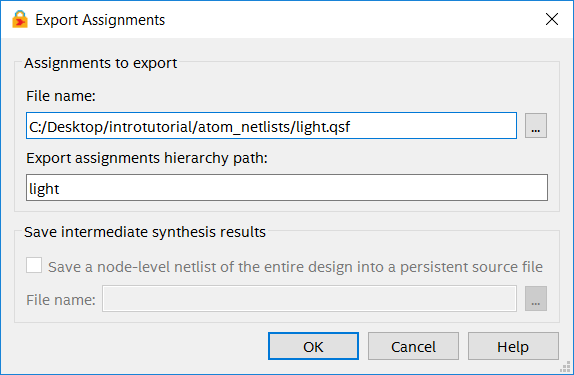
\includegraphics[scale=0.65]{figures/figure26.png}
   \caption{Exporting the pin assignment.} 
	 \label{fig:26}
	 \end{center}
\end{figure}

You can import a pin assignment by choosing {\sf Assignments $>$ Import Assignments}. 
This opens the dialogue in Figure~\ref{fig:27} to select the file to import. 
Type the name of the file, including the {\it qsf} extension and the full path
to the directory that holds the file, in the File Name box and press {\sf OK}.
Of course, you can also browse to find the desired file.
 
\begin{figure}[H]
   \begin{center}
      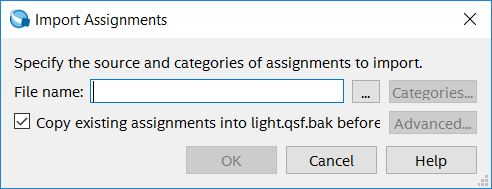
\includegraphics[scale=0.65]{figures/figure27.png}
   \caption{Importing the pin assignment.} 
	 \label{fig:27}
	 \end{center}
\end{figure}


% Additional to pin assignments sections.
For convenience when using large designs, all relevant pin assignments for the 
DE-series board are given in individual files. For example, the DE1-SoC pin assignments 
can be found in the {\it DE1\_SoC.qsf} file, which is available from Intel's FPGA University
Program website.
This file uses the names found in the {\it DE1-SoC User Manual}.
If we wanted to make the pin assignments for our example circuit by importing
this file, then we would have to use the same names in our 
Block Diagram/Schematic design file;
namely, {\it SW[0]}, {\it SW[1]} and {\it LEDG[0]} for 
{\it x1}, {\it x2} and {\it f}, respectively.
Since these signals are specified in the {\it DE1\_SoC.qsf} file
as elements of vectors {\it SW} and {\it LEDG}, we must refer to them in the same
way in our design file. For example, in the {\it DE1\_SoC.qsf} 
file the 10 toggle switches are called {\it SW[9]} to {\it SW[0]}.
In a design file they can also be referred to as a vector {\it SW[9..0]}.
%%%%%%%%%%%%%%%%%%%%%%%%%

%%%%%%%%%%%%%%%%%%%%%%%%%
% Programming and Configuring
\newpage
\section{Programming and Configuring the FPGA Device}

The FPGA device must be programmed to implement the designed 
circuit. The required configuration file is generated by the Quartus Prime 
Compiler's Assembler module. Each DE-series board allows the configuration to 
be done in two different ways, known as JTAG* and AS modes.
The configuration data is transferred from the host computer (which runs the 
Quartus Prime software) to the board by means of a cable that connects 
a USB port on the host computer to the {\it USB-Blaster} connector on the board.
To use this connection, it is necessary to have the USB-Blaster (II) driver 
installed. If this driver is not already installed, consult the 
tutorial {\it Getting Started with the Terasic DE-Series Boards},
available on {\small \href{https://www.fpgacademy.org/tutorials.html} {FPGAcademy.org}},
for information about installing the driver. You can also search on the Internet for a
topic such as ``Installing USB Blaster driver''.
Before using the board, make sure that the USB cable is properly connected
and that the board is powered on.
 
In the JTAG mode, the configuration data is loaded directly
into the FPGA device. The acronym JTAG stands for Joint Test Action Group. 
This group defined a simple way for testing digital circuits and loading data 
into them, which became an IEEE* standard. If the FPGA is configured in 
this manner, it will retain its 
configuration as long as the power remains turned on. 
The configuration information is lost when the power is turned off.
The second possibility is to use the Active Serial (AS) mode.
In this case, a configuration device that includes some flash memory is used 
to store the configuration data. Quartus Prime software places the configuration 
data into the configuration device on the DE-series board. Then, this data is loaded 
into the FPGA upon power-up or reconfiguration.
Thus, the FPGA need not be configured by the Quartus Prime software if the power 
is turned off and on. 
The choice between the two modes is made by switches on the DE-series 
board. Consult your manual for the location of this switch on your DE-series board. The boards should be set to JTAG mode by default.
This tutorial discusses only the JTAG programming mode.

\subsection{JTAG* Programming for the DE1-SoC Board, DE0-Nano-SoC, DE10-Nano, and DE10-Standard}

For the DE1-SoC Board, DE0-Nano-SoC, DE10-Nano, and DE10-Standard boards, 
the following steps should be used for programming.  Select {\sf Tools $>$ Programmer} to reach 
the window in Figure~\ref{fig:SoC1}. If the {\it SOCVHPS} device shown in the figure is missing, 
then you need to add it. Click on the {\sf Add Device} menu, and then look for the {\it SOCVHPS}
device under the \textit{Soc Series V} family.
Now it is necessary to specify the programming hardware and 
the mode that should be used. If not already chosen by default, 
select JTAG in the {\sf Mode} box.  The required programming hardware is called {\it DE-SoC}. If
this hardware is not chosen by default as the programming
hardware, then press the {\sf Hardware Setup...} button and select the {\it DE-SoC} in the 
window that pops up, as shown in Figure~\ref{fig:SoC2}.\footnote{In some versions of the
Microsoft Windows operating system the drivers provided with older versions of the Quartus
Prime software might fail to install. In such cases, no programming Hardware will be available to
the Quartus Programmer. One approach to solving such an issue is to download and install the 
drivers that are provided with a more recent version of the Quartus Prime software.
If you install a version of Quartus Prime into a folder named
\texttt{Qdir}, then the drivers that come with this version can be found in the sub-folder
\texttt{Qdir/quartus/drivers}. The driver for the DE-SoC hardware is called {\it
USB-Blaster-II}.}  

Observe that the configuration file {\it light.sof} in directory {\it output\_files} is 
listed in the window in
Figure~\ref{fig:SoC1}. If the file is not already listed, then click {\sf Add File} 
and select it.  This is a binary file produced by the Compiler's Assembler module, 
which contains the data needed to configure the FPGA device.
The extension {\it .sof} stands for SRAM Object File.
Ensure the {\sf Program/Configure} box is checked.
This setting is used to select the FPGA in the Cyclone V SoC chip for programming.

Press {\sf Start} in the Programmer to program the FPGA device.  An LED on the board will 
light up while the FPGA device is being programmed. 
If you see an error reported by Quartus Prime software indicating that
programming {\it failed}, then check to ensure that the board is properly powered on.
Also, as mentioned above, if the {\it SOCVHPS} device is not shown as in Figure~\ref{fig:SoC1}, 
click {\sf Add Device $>$ SoC Series V $>$ SOCVHPS}, and then click {\sf OK} to add it.
Some boards use the device order shown in Figure~\ref{fig:SoC1}, and others use the
opposite order. If programming of your board failed, try reversing the order
from what is shown in the figure, by clicking on a device and then clicking 

\includegraphics[scale=.55]{figures/icon14.png} or 

\includegraphics[scale=.55]{figures/icon13.png}.

\begin{figure}[H]
   \begin{center}
      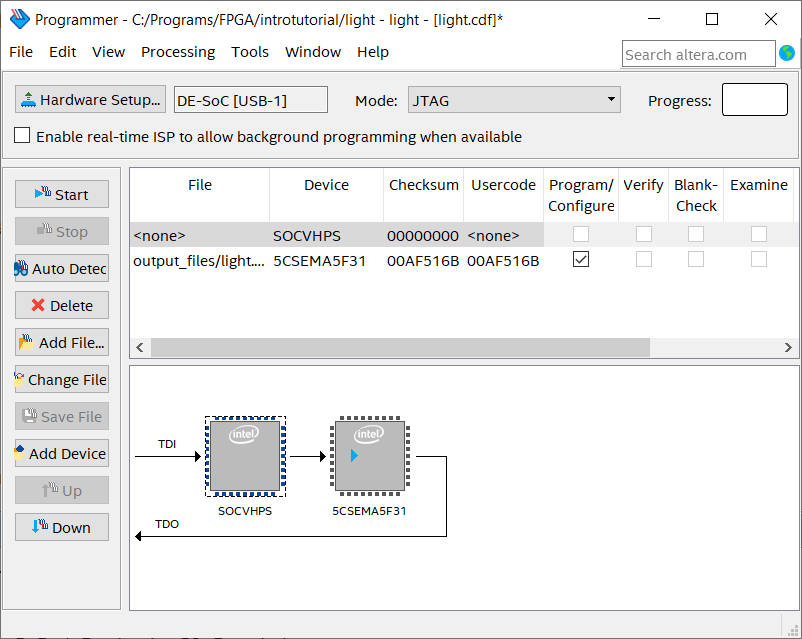
\includegraphics[width=0.65\textwidth]{figures/figureSoC1.png}
   \caption{The Programmer window.} 
	 \label{fig:SoC1}
	 \end{center}
\end{figure}

\begin{figure}[H]
   \begin{center}
      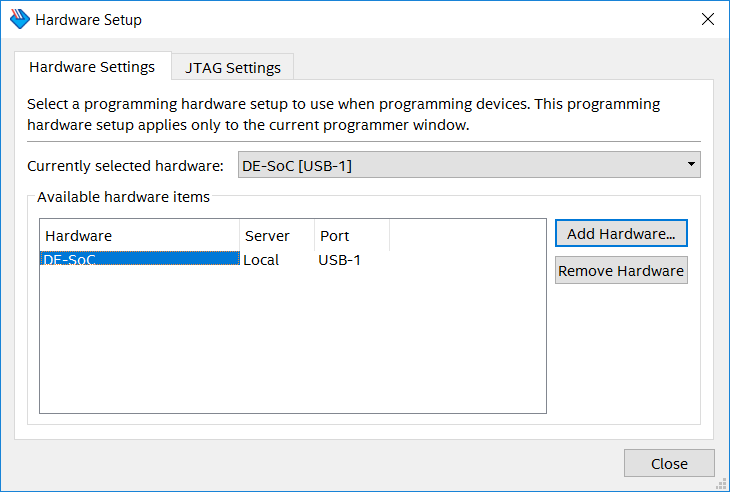
\includegraphics[scale=0.65]{figures/figureSoC2.png}
   \caption{The Hardware Setup window.} 
	 \label{fig:SoC2}
	 \end{center}
\end{figure}

\subsection{JTAG* Programming for the DE0-CV, DE0-Nano, DE10-Lite, and DE2-115 Boards}

For the DE0-CV, DE0-Nano, DE10-Lite, and DE2-115 Boards, the
programming and configuration task is performed as follows. 
Select {\sf Tools $>$ Programmer} to reach the window in Figure~\ref{fig:38}.
Here it is necessary to specify the programming hardware and 
the mode that should be used. If not already chosen by default, 
select JTAG in the Mode box.
Also, if the USB-Blaster is not chosen by default, press the 
{\sf Hardware Setup...} button and select the USB-Blaster in the window
that pops up, as shown in Figure~\ref{fig:39}. \footnote{In some versions of the
Microsoft Windows operating system the USB-Blaster driver provided with older versions of the 
Quartus Prime software might fail to install. In such cases, no programming Hardware will be 
available to the Quartus Programmer. One approach to solving such an issue is to download and 
install the USB-Blaster driver that is provided with a more recent version of the Quartus 
Prime software. If you install a version of Quartus Prime into a folder named
\texttt{Qdir}, then the drivers that come with this version can be found in the sub-folder
\texttt{Qdir/quartus/drivers}.}  

\begin{figure}[H]
   \begin{center}
      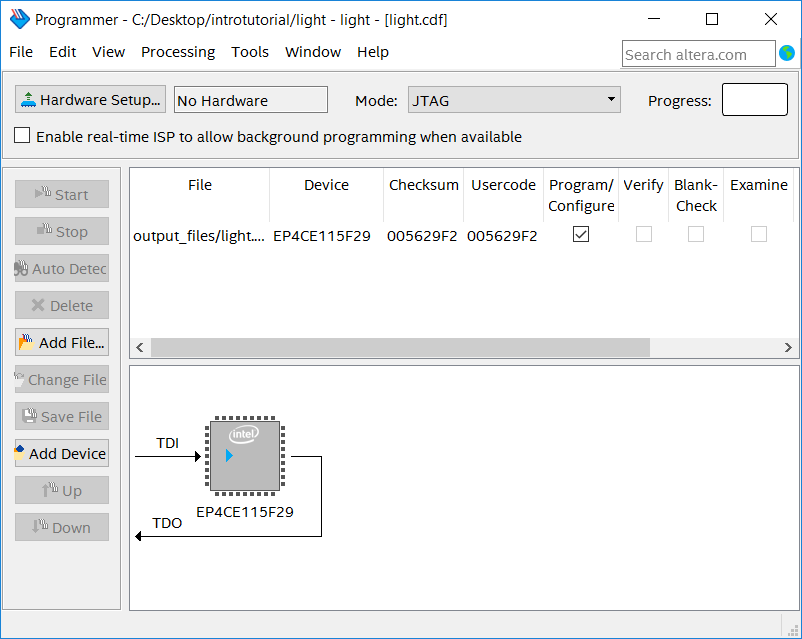
\includegraphics[scale=0.65]{figures/figure38.png}
   \caption{The Programmer window.} 
	 \label{fig:38}
	 \end{center}
\end{figure}

Observe that the configuration file {\it light.sof} is listed in the window in
Figure~\ref{fig:38}. If the file is not already listed, then click {\sf Add File}
and select it.
This is a binary file produced by the Compiler's Assembler module, 
which contains the data needed to configure the FPGA device.
The extension {\it .sof} stands for SRAM Object File.
Ensure the {\sf Program/Configure} check box is ticked, as shown in Figure~\ref{fig:38}.

\begin{figure}[H]
   \begin{center}
      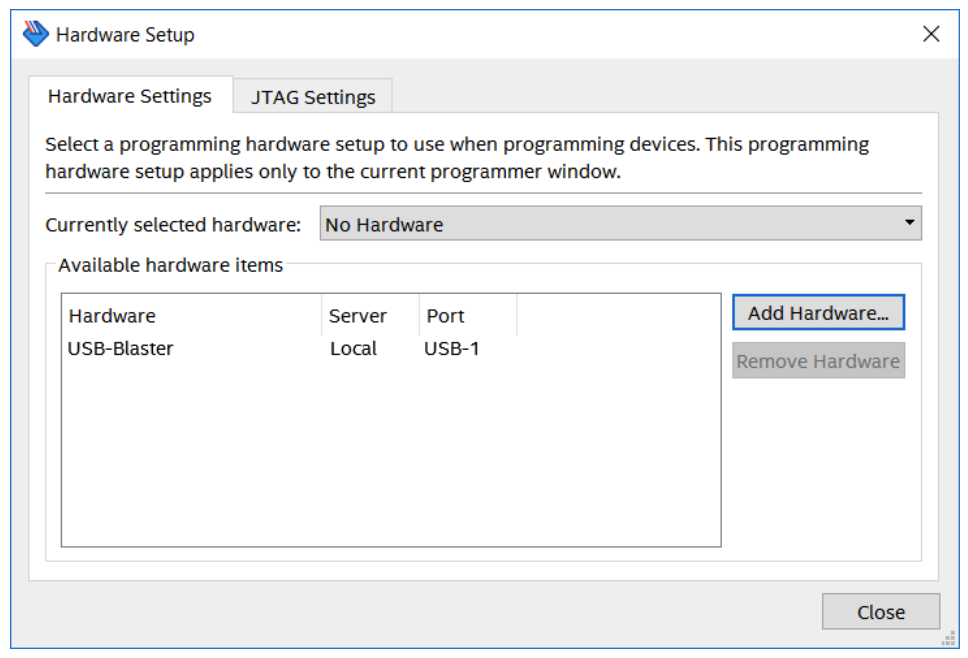
\includegraphics[scale=0.65]{figures/figure39.png}
   \caption{The Hardware Setup window.} 
	 \label{fig:39}
	 \end{center}
\end{figure}

Now, press {\sf Start} in the window in Figure~\ref{fig:38}.
An LED on the board will light up corresponding to the programming operation.
If you see an error reported by Quartus Prime software indicating that
programming failed, then check to ensure that the board is properly powered on.


%%%%%%%%%%%%%%%%%%%%%%%%%

%%%%%%%%%%%%%%%%%%%%%%%%%
% Testing Designed Circuit
\section{Testing the Designed Circuit}

Before implementing the designed circuit in the FPGA chip on the DE-series board, it is
prudent to simulate it to ascertain its correctness. While not covered in this tutorial,
users may use software such as {\it ModelSim} or other simulation environments to test the 
circuit in simulation. Simulation of a circuit often provides a comprehensive view of the 
circuit's functionality, and can help users easily find bugs within the circuit's logic 
without having to touch hardware.

Having downloaded the configuration data into the FPGA device, you can now
test the implemented circuit.  Try all four valuations of the input variables
$x_1$ and $x_2$, by setting the corresponding states of the switches
$SW_1$ and $SW_0$. Verify that the circuit implements the truth table
in Figure~\ref{fig:11}.

If you want to make changes in the designed circuit, first close the Programmer window.
Then make the desired changes in the \typeName{} design file, compile the circuit,
and program the board as explained above.

%%%%%%%%%%%%%%%%%%%%%%%%%

%%%%%%%%%%%%%%%%%%%%%%%%%
% Copyright

%\newcommand{\datePublished}{Mar 2022}

\newcommand{\versnum}{21.1} %version number quartus/AMP
\newcommand{\quartusname}{Quartus\textsuperscript{\textregistered} Prime}	
\newcommand{\textBar}{For \quartusname{} \versnum{}}
\newcommand{\thisyear}{2022 } %for copyright
\newcommand{\company}{FPGAcademy.org}
\newcommand{\longteamname}{FPGAcademy.org}
\newcommand{\teamname}{FPGAcademy}
\newcommand{\website}{FPGAcademy.org}

\newcommand{\productAcronym}{AMP}
\newcommand{\productNameShort}{Monitor Program}

\newcommand{\productNameMedTM}{Monitor Program}
\newcommand{\productNameMed}{Monitor Program}

%\newcommand{\headerLogoFilePath}[1]{#1/FPGAcademy.png}



%%%%%%%%%%%%%%%%%%%%%%%%%%%%%%%%%%%%%%%%
%%% FPGAcademy Copyright Information %%%
%%%%%%%%%%%%%%%%%%%%%%%%%%%%%%%%%%%%%%%%

%Always put the copyright on a new page (clear page), with some vertical space from top
\clearpage
\vspace{1in}

\noindent

Copyright {\copyright} FPGAcademy.org. All rights reserved. FPGAcademy and the FPGAcademy logo are trademarks of  FPGAcademy.org.  This document is being provided on an ``as-is'' basis and as an accommodation and therefore all warranties, representations or guarantees of any kind (whether express, implied or statutory) including, without limitation, warranties of merchantability, non-infringement, or fitness for a particular purpose, are specifically disclaimed.

%FPGAcademy assumes no responsibility or liability arising out of the application or use of any information,  product,  or  service  described  herein  except  as  expressly  agreed  to  in  writing  by  FPGAcademy.



**Other names and brands may be claimed as the property of others.



%%%%%%%%%%%%%%%%%%%%%%%%%

\end{document}
% Document Ends
%%%%%%%%%%%%%%%%%%%%%%%%%
